% analisi_dei_requisiti/analisi_dei_requisiti.tex

% **************************************************
% Macro specifiche per il documento corrente
% **************************************************
% Nome
\newcommand{\docName}{Analisi dei requisiti}
% Nome file
\newcommand{\docFileName}{analisi\_dei\_requisiti.2.0.pdf}
% Versione
\newcommand{\docVers}{2.0}
% Data creazione
\newcommand{\creationDate}{2012-12-03}
% Data ultima modifica
\newcommand{\modificationDate}{2013-01-18}
% Stato in {Approvato, Non approvato}
\newcommand{\docState}{Approvato}
% Uso in {Interno, Esterno}
\newcommand{\docUsage}{Esterno}
% Destinatari da specificare come nome1\\ &nome2\\ ecc.
\newcommand{\docDistributionList}{Prof. Tullio Vardanga\\ & Prof. Riccardo Cardin\\ & Dott. Gregorio Piccoli \\& Team \team{}}
% Redattori da specificare come nome1\\ &nome2\\ ecc.
\newcommand{\docAuthors}{Andrea Meneghinello \\& Andrea Rizzi\\& Diego Beraldin\\& Elena Zecchinato\\& Marco Schivo\\& Riccardo Tresoldi\\& Stefano Farronato}
% Approvato da
\newcommand{\approvedBy}{Andrea Meneghinello}
% Verificatori
\newcommand{\verifiedBy}{Andrea Rizzi\\}
% Perscorso (relativo o assoluto) che punta alla directory contenente shared/
% come sua sottodirectory (per comodità chiamiamola 'doc root').
\newcommand{\docRoot}{..}
% definire se si vuole l'indice delle tabelle
\def\INDICETABELLE{false}
% definire se si vuole l'indice delle figure
\def\INDICEFIGURE{true}

% importa il preambolo condiviso da tutti i documenti
% shared/preamble.tex
%
% Questo documento contiene la parte del preambolo condivisa e viene pertanto
% richiamato nel 'master' di tutti i documenti di progetto.  Al suo interno
% contiene le inclusioni (e le configurazioni) di tutti i package richiesti per
% la compilazione dei documenti, le macro di carattere generale e la definizione
% degli stili di pagina.

\documentclass[a4paper,10pt,openright]{article}

% **************************************************
% Macro generiche
% **************************************************
\newcommand{\team}{Software Synthesis}                    % chi siamo
\newcommand{\email}{software.synthesis@gmail.com}         % e-mail
\newcommand{\caName}{}                                    % titolo capitolato
\newcommand{\caDescr}{}                                   % descrizione
\newcommand{\inglese}[1]{\textit{#1}}

% **************************************************
% Codifica e lingua dei documenti
% **************************************************
\usepackage[utf8x]{inputenc}                              % codifica caratteri dei documenti sorgenti
\usepackage[english,italian]{babel}                       % localizzazione ai fini di sillabazione e cross-references
\usepackage[T1]{fontenc}                                  % codifica font di output

% **************************************************
% Definizione geometria della pagina
% **************************************************
\usepackage[a4paper,head=4cm,top=4.5cm,bottom=3cm,left=3cm,right=3cm,bindingoffset=5mm]{geometry}

% *************************************************
% Intestazioni e piè di pagina personalizzati
% *************************************************
\usepackage{fancyhdr}
% stile normale
\fancypagestyle{normal}{
\fancyhead{}                                              % intestazione
\fancyhead[RE,RO]{
\begin{picture}(0,0)
  \put(-410,0){
\includegraphics[width=1.02\textwidth]{header_logo}}
  \put(-410,10){\sffamily\large\leftmark}
\end{picture}
\vspace{-4pt}
}
\renewcommand{\headrulewidth}{.4pt}                       % riga sotto l'intestazione
\cfoot{}                                                  % piè di pagina
\fancyfoot[RO,LE]{\sffamily
  pag.~\thepage{} di \pageref{LastPage}}                  % a dx nelle pag. dispari e a sx in quelle pari
\fancyfoot[RE,LO]{\sffamily\docFileName{} -- v.\docVers}
\renewcommand{\footrulewidth}{.4pt}                       % riga sopra il piè di pagina
}
% stile per gli indici
\fancypagestyle{toc}{
\fancyhead{}                                              % intestazione
\fancyhead[RE,RO]{
\begin{picture}(0,0)
  \put(-410,0){
\includegraphics[width=1.02\textwidth]{header_logo}}
\end{picture}
}
\renewcommand{\headrule}{}                                % nessuna riga sotto l'intestazione
\cfoot{}                                                  % piè di pagina
\fancyfoot[RO,LE]{\sffamily\thepage{}}                    % a dx nelle pag. dispari e a sx in quelle pari
\fancyfoot[RE,LO]{\sffamily\docFileName{} -- v.\docVers}
\renewcommand{\footrulewidth}{.4pt}                       % riga sopra il piè di pagina
}

\pagestyle{fancy}                                         % premetto: non so usare bene le marche:
\renewcommand{\sectionmark}[1]{\markboth{#1}{#1}}         % se qualcuno ha idee migliori si faccia avanti!

% **************************************************
% Tabelle
% **************************************************
\usepackage{tabularx}                                     % tabelle di larghezza fissa con una o più colonne variabili
\usepackage{multirow}                                     % colonne con colonne che si estendono per più righe
\usepackage{booktabs}                                     % per inserire l'ambiente table e le righe orizz. nelle tabelle
\usepackage{longtable}			                          % tabelle oltre i limiti di pagina

% **************************************************
% Cross-references e collegamenti ipertestuali
% **************************************************
\usepackage[hidelinks]{hyperref}
\hypersetup{%
  colorlinks=false, linktocpage=false, pdfborder={0,0,0}, pdfstartpage=3, pdfstartview=FitV,%
  urlcolor=Cyan, linkcolor=Cyan, citecolor=Black, %pagecolor=Black,%
  pdftitle={\docName}, pdfauthor={\team}, pdfsubject={}, pdfkeywords={},%
  pdfcreator={pdflatex}, pdfproducer={pdflatex with hyperref package}%
}

% **************************************************
% Immagini e grafica
% **************************************************
\usepackage{graphicx}                                     % supporto ad aspetti avanzati delle immagini
\graphicspath{{\docRoot/pics/}}                           % percorso contenente tutti i file immagini
\usepackage{color}                                        % permette di colorare facilmente il testo

% **************************************************
% Altri pacchetti opzionali
% **************************************************     
\usepackage{lastpage}                                     % per sapere il numero totale di pagine
\usepackage{lipsum}                                       % genera "dummy text" per prove di impaginazione
\usepackage{eurosym}                                      % per il simbolo dell'euro usare \EUR{x} dove x è l'importo


% Fine del preambolo e inizio del documento
\begin{document}

% Inclusione della prima pagina
% shared/firstpage.tex
%
% Questo documento definisce il contenuto della prima pagina, che si suppone
% essere uguale in tutti i documenti.  Oltre al logo e al titolo, la prima
% pagina contiene i metadati relativi al documento in cui viene inclusa.


% rimuove intestazioni e piè di pagina
\pagestyle{empty}

\begin{center}

% logo del gruppo

\includegraphics[width=1.5\textwidth]{logo}

\vspace{1in}

% titolo del documento
{\Huge\bfseries \docName}

\vspace{1in}

% tabella riepilogativa
\begin{tabularx}{.7\textwidth}{>{\bfseries\sffamily}l>{\sffamily}l}
\toprule
\multicolumn{2}{>{\sffamily}c}{Informazioni sul documento}\\
\midrule
Nome file:            & \docFileName\\
Versione:             & \docVers\\
Data creazione:       & \creationDate\\
Data ultima modifica: & \modificationDate\\
Stato:                & \docState\\
Uso:                  & \docUsage\\
Redattori:            & \docAuthors\\
Approvato da:         & \approvedBy\\
Verificatori:         & \verifiedBy\\
\bottomrule
\end{tabularx}

\end{center}

\newpage


% Storico delle modifiche
\section*{Storia delle modifiche}
\begin{center}
\begin{longtable}{lp{.32\textwidth}lll}
\toprule
Versione & Descrizione intervento & Membro & Ruolo & Data\\
\midrule % inserire qui il contenuto della tabella

2.0 & Approvazione del documento & Andrea Meneghinello & Responsabile & 2013-01-18\\
1.11 & Verifica lessicale e grammaticale del documento & Andrea Rizzi & Verificatore & 2013-01-18\\
1.10 & Correzione errori rilevati dal verificatore & Marco Schivo & Analista & 2013-01-17\\
1.9 & Verifica corrispondenza e coerenza dei dati nelle tabelle e diagrammi & Andrea Rizzi & Verificatore & 2013-01-15\\
1.8 & Inserimento sezione Requisiti-Test & Marco Schivo & Analista & 2013-01-16\\
1.7 & Revisione modalità di visualizzazione codice dei requisiti, aggiunta tabella tracciamento requisiti-casi d'uso. & Marco Schivo & Analista & 2013-01-15\\
1.6 & Aggiunti vincoli riportati nel capitolato ma non riportati in RR, aggiunti riferimenti espliciti ai codici dei corrispondenti casi d'uso. & Diego Beraldin & Analista & 2013-01-15\\
1.5 & Correzione UC2.0 e UC2.5 Correzione RUFO 1.0.0 RUFO2.0.0 RUFO 3.0.0 & Marco Schivo & Analista & 2013-01-14\\
1.4 & Specializzato UC2.2. Correzione errori ortografici. Correzione UC2.1. Correzione UC2.5. & Diego Beraldin & Analista & 2013-01-12\\
1.3 &  Modificata Sez. ``Assunzioni e prerequisiti''. Modificato UC1 & Diego Beraldin & Analista & 2013-01-12\\
1.2 & Correzione errori rilevati in RR: aggiornamento tabella delle modifiche con l'aggiunta dei ruoli. Aggiunta la lista di distribuzione. Aggiunto sommario. Aggiornati i riferimenti normativi. & Diego Beraldin & Analista & 2013-01-12\\
1.1 & Correzione errori ortografici non rilevati. & Diego Beraldin & Analista & 2013-01-09\\
1.0 & Approvazione documento. & Elena Zecchinato & Responsabile & 2012-12-18\\
0.13 & Verifica dell'intero documento. & Diego Beraldin & Verificatore & 2012-12-18\\
0.12 & Correzione casi d'uso errati. Aggiunta requisiti mancanti. Fine stesura documento. & Andrea Rizzi & Analista & 2012-12-17\\
0.11 & Seconda stesura dei casi d'uso e loro inserimento nel sistema \manager. & Riccardo Tresoldi & Analista & 2012-12-15\\
0.10 & Correzione requisiti errati. Correzione casi d'uso errati. & Stefano Farronato & Analista & 2012-12-14\\
0.9 & Seconda stesura dei requisiti e loro inserimento nel sistema \manager. & Andrea Meneghinello & Analista & 2012-12-13\\
0.8 & Incontro con il proponente. Stesura dei requisiti emersi. Correzione requisiti errati. & Riccardo Tresoldi & Analista & 2012-12-10\\
0.7 & Verifica documento fino alla versione 0.4. Correzione errori nel punto ``funzionalità''. & Marco Schivo & Verificatore & 2012-12-08\\
0.6 & Prima stesura dei casi d'uso e loro inserimento nel sistema \manager. Stesura del punto ``Requisiti'' (introduzione) & Riccardo Tresoldi & Analista & 2012-12-07\\
0.5 & Continuazione stesura dei requisiti e loro inserimento nel sistema \manager. Correzione requisiti errati. & Diego Beraldin & Analista & 2012-12-06\\
0.4 & Prima stesura dei requisiti e loro inserimento nel sistema \manager. & Andrea Rizzi & Analista & 2012-12-05\\
0.3 & Stesura del punto ``Funzionalità'' e ``Assunzioni e prerequisiti''. & Diego Beraldin & Analista & 2012-12-04\\
0.2 & Stesura del punto ``Riferimenti'' e ``Descrizione generale''. & Riccardo Tresoldi & Analista & 2012-12-03\\
0.1 & Creazione del documento e stesura del punto ``Scopo del documento''. & Andrea Rizzi & Analista & 2012-12-03\\
\bottomrule
\end{longtable}
\end{center}
\newpage

% inclusione dell'indice
% shared/toc.tex
%
% Questo file contiene le istruzioni che generano l'indice o gli indici del
% documento (utile nel caso in cui decidessimo di avere anche un indice delle
% tabelle e/o un indice delle figure).

\pagestyle{toc}
\pagenumbering{roman}

\tableofcontents

\newpage


% Alcuni aggiustamenti per le pagine
\pagenumbering{arabic}
\setcounter{page}{1}
\pagestyle{normal}

% Qui ha inizio il documento vero e proprio...

\begin{abstract}
Il presente documento, nasce con la necessità di evidenziare i requisiti che costituiscono il sistema e i casi d'uso associati. Inoltre viene proposta la tabella di tracciamento requisiti-casi e requisiti-fonti.
\end{abstract}

\newpage

\section{Introduzione}
\subsection{Scopo del prodotto}
\purpose

\subsection{Scopo del documento}
Il presente documento riporta il risultato dell'attività di analisi dei requisiti svolta dal gruppo \team{} in fase preliminare, vale a dire un insieme di requisiti -- in parte esplicitati nel testo del capitolato C1, in parte emersi durante incontri con il committente Zucchetti S.r.l., in parte inferiti dal dominio e in parte auto-imposti dal gruppo -- che il prodotto software è tenuto a soddisfare in termini funzionali, prestazionali, qualitativi e dichiarativi.

Il comportamento del sistema osservabile dall'utente finale, in conformità con i requisiti sopra enunciati, è riportato secondo il formalismo noto come diagrammi dei casi d'uso. La corrispondenza fra casi d'uso e requisiti è illustrata mediante la tabella riportata nella sezione~\ref{sec:tracciamento}.
%TODO: aggiungere riferimenti incrociati e non basarsi su numeri hard-coded qui dentro

\subsection{Glossario}
\glossaryIntro

\clearpage
\section{Riferimenti}

\subsection{Normativi}
\begin{itemize}
%\item[] verbale \textit{verbale\_incontro\_2012-12-11.pdf} allegato;
\item[] \textit{piano\_di\_qualifica.3.0.pdf} allegato.
\item[] \textit{norme\_di\_progetto.3.0.pdf} allegato.
\end{itemize}

\subsection{Informativi}
\begin{itemize}
\item[] Capitolato d'appalto: \caName{}, v1.0, redatto e rilasciato dal proponente Zucchetti s.r.l. reperibile all'indirizzo \url{http://www.math.unipd.it/~tullio/IS-1/2012/Progetto/C1.pdf};
\item[] testo di consultazione: \textit{Software Engineering (8th edition) Ian Sommerville, Pearson Education | Addison Wesley};
\item[] \textit{glossario.3.0.pdf} allegato.
\end{itemize}

\clearpage
\section{Descrizione generale}

\subsection{Contesto di utilizzo}
Il sistema software realizzato nell'ambito del progetto \caName{} si configura come una piattaforma di comunicazione fra utenti connessi alla rete. Oggetto della condivisione -- poiché ``comunicare'' letteralmente significa ``mettere in comune'' -- saranno non solo flussi audio/video, secondo le modalità tipiche della (video)chiamata via \inglese{softphone}, ma anche file e documenti presenti in locale, per i quali è previsto tanto il trasferimento quanto la condivisione delle modifiche in tempo reale.\\
Dal punto di vista dell'utente, \caName{} si configura inoltre come un applicativo fruibile attraverso la sola mediazione di un \underline{browser} per la navigazione web, senza necessità di installazione di alcun programma \inglese{stand-alone} sul proprio sistema né di \underline{plugin} per il browser forniti da \team{} o da terze parti.\\
Al fine di gestire l'utenza è prevista la realizzazione di una parte di \inglese{back-end} da installare in un \underline{server} sotto il controllo del fornitore del servizio agli utenti. L'installazione dell'applicativo lato {server} è prevista in un ambiente \underline{TomCat}.

\subsection{Utente finale}
Il modello di utente finale di riferimento prevede la disponibilità di una connessione a Internet funzionante e di un browser di ultima generazione in grado di supportare lo standard \underline{WebRTC}.\\
Fra i prerequisiti non figura il possesso di conoscenze particolari estranee alla comune esperienza di navigazione web (in particolare, l'eventuale confidenza con sistemi esistenti di telefonia via internet non rientra nelle assunzioni).

\subsection{Funzionalità}
Le funzionalità offerte dal prodotto agli utenti finali possono essere suddivise in due categorie principali:
\begin{itemize}
  \item gestione di scambi di informazioni in tempo reale, in particolare
  \begin{itemize}
  \item[--] comunicazione audio e audio/video tra due (o più) utenti;
  \item[--] chat testuale;
  \item[--] condivisione di risorse (ad esempio lavagna grafica, schermo e documenti PDF). 
  \end{itemize}
  \item scambio di informazioni asincrone 
  \begin{itemize}
  \item[--] segreteria (sia per messaggi vocali che videomessaggi);
  \item[--] trasferimento file.
  \end{itemize}
\end{itemize}
A integrazione e supporto di tali funzionalità di base è previsto lo sviluppo di funzionalità secondarie quali l'autenticazione degli utenti, la gestione della rubrica, la visualizzazione di metadati sulle connessioni e la possibilità di mantenere un registro storico delle attività realizzate mediante il sistema.

\subsection{Assunzioni e prerequisiti}
%In fase di \underline{\inglese{deployment}} si presuppone che l'installatore presso il committente sia in possesso delle competenze necessarie per l'installazione e la configurazione della parte server del sistema.
Si assume che l'utente sia in possesso di una connessione a internet funzionante al fine di instaurare la comunicazione. È altresì assunto implicitamente l'utilizzo di un browser con supporto a WebRTC.

\clearpage
%da qua in poi mi affido al software di stampa automatico
\newpage\section{Diagrammi dei casi d'uso}

\subsection{UC1: Login e registrazione}
\begin{figure}[H]
\begin{center}
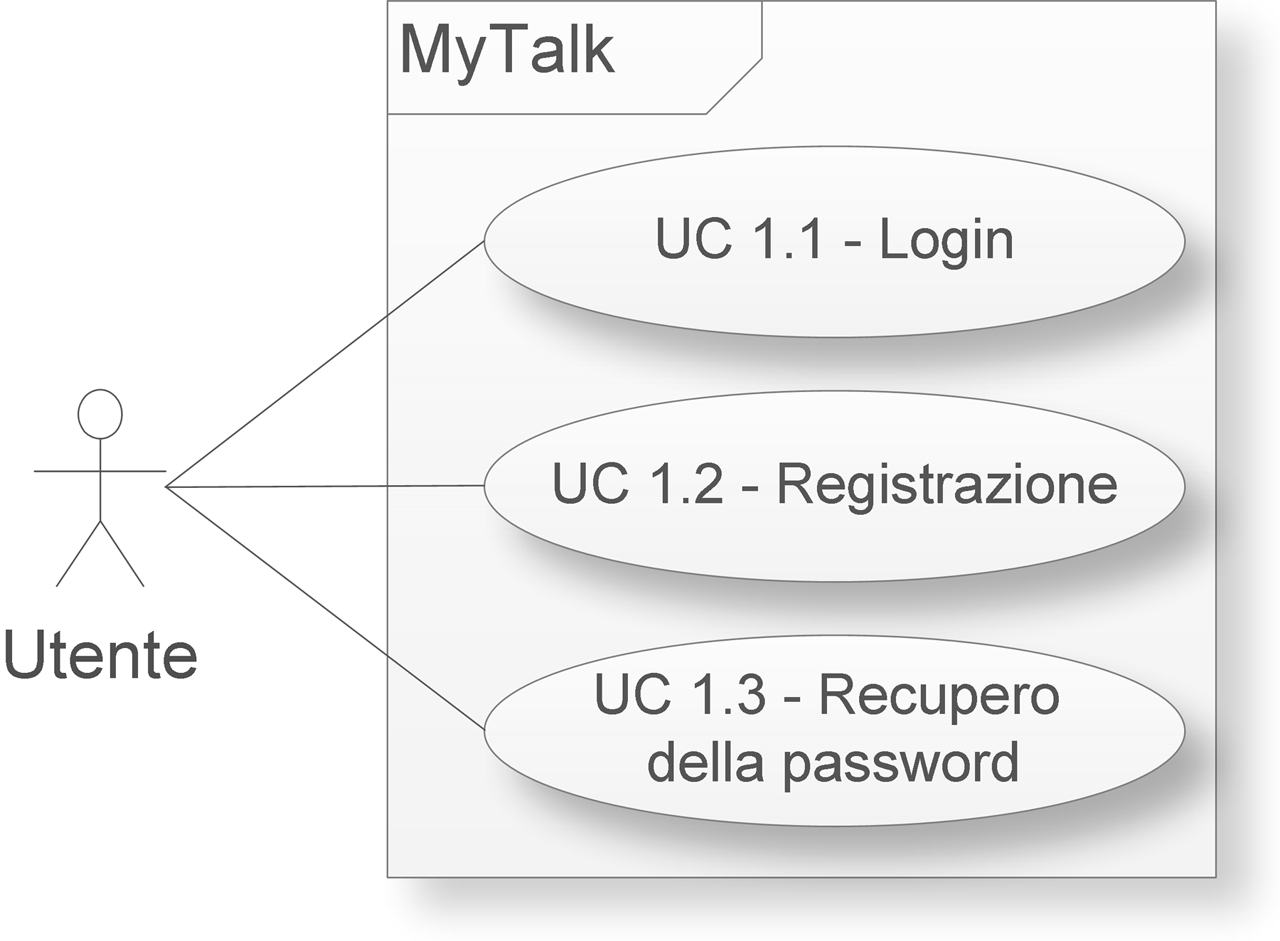
\includegraphics[width=.8\textwidth]{UC1}
\caption{}\label{fig:}
\end{center}
\end{figure}
\begin{description}
\item{\scshape\bfseries Attori principali:}Utente.
\item{\scshape\bfseries Scopo e descrizione:} L'utente può effettuare l'accesso al sistema mediante la procedura di autenticazione se registrato (UC1.1), recuperare la password dimenticata (UC1.3) oppure può provvedere alla propria registrazione (UC1.2), quindi effettuare successivamente l'accesso al sistema (UC1.1).
\item{\scshape\bfseries Precondizione:} Il sistema MyTalk è attivo e funzionante, le infrastrutture di rete sono attive.
\item{\scshape\bfseries Postcondizione:} L'utente si trova in uno di questi casi: ha avviato la procedura per l'autenticazione al sistema (UC1.1), oppure ha avviato la procedura per per la registrazione nel sistema (UC1.2), oppure ha avviato la procedura per il recupero della password dimenticata (UC1.3).
\item{\scshape\bfseries Illustrazione scenario principale:} L'utente può decidere di avviare la procedura di autenticazione al sistema (UC1.1), altrimenti se non ricorda le credenziali, può avviare la procedura per il recupero della password (UC1.3). Invece se l'utente sa di non essere registrato nel sistema, può avviare la procedura di registrazione (UC1.2).
\end{description}

\subsection{UC1.1: Login utente}
\begin{figure}[H]
\begin{center}
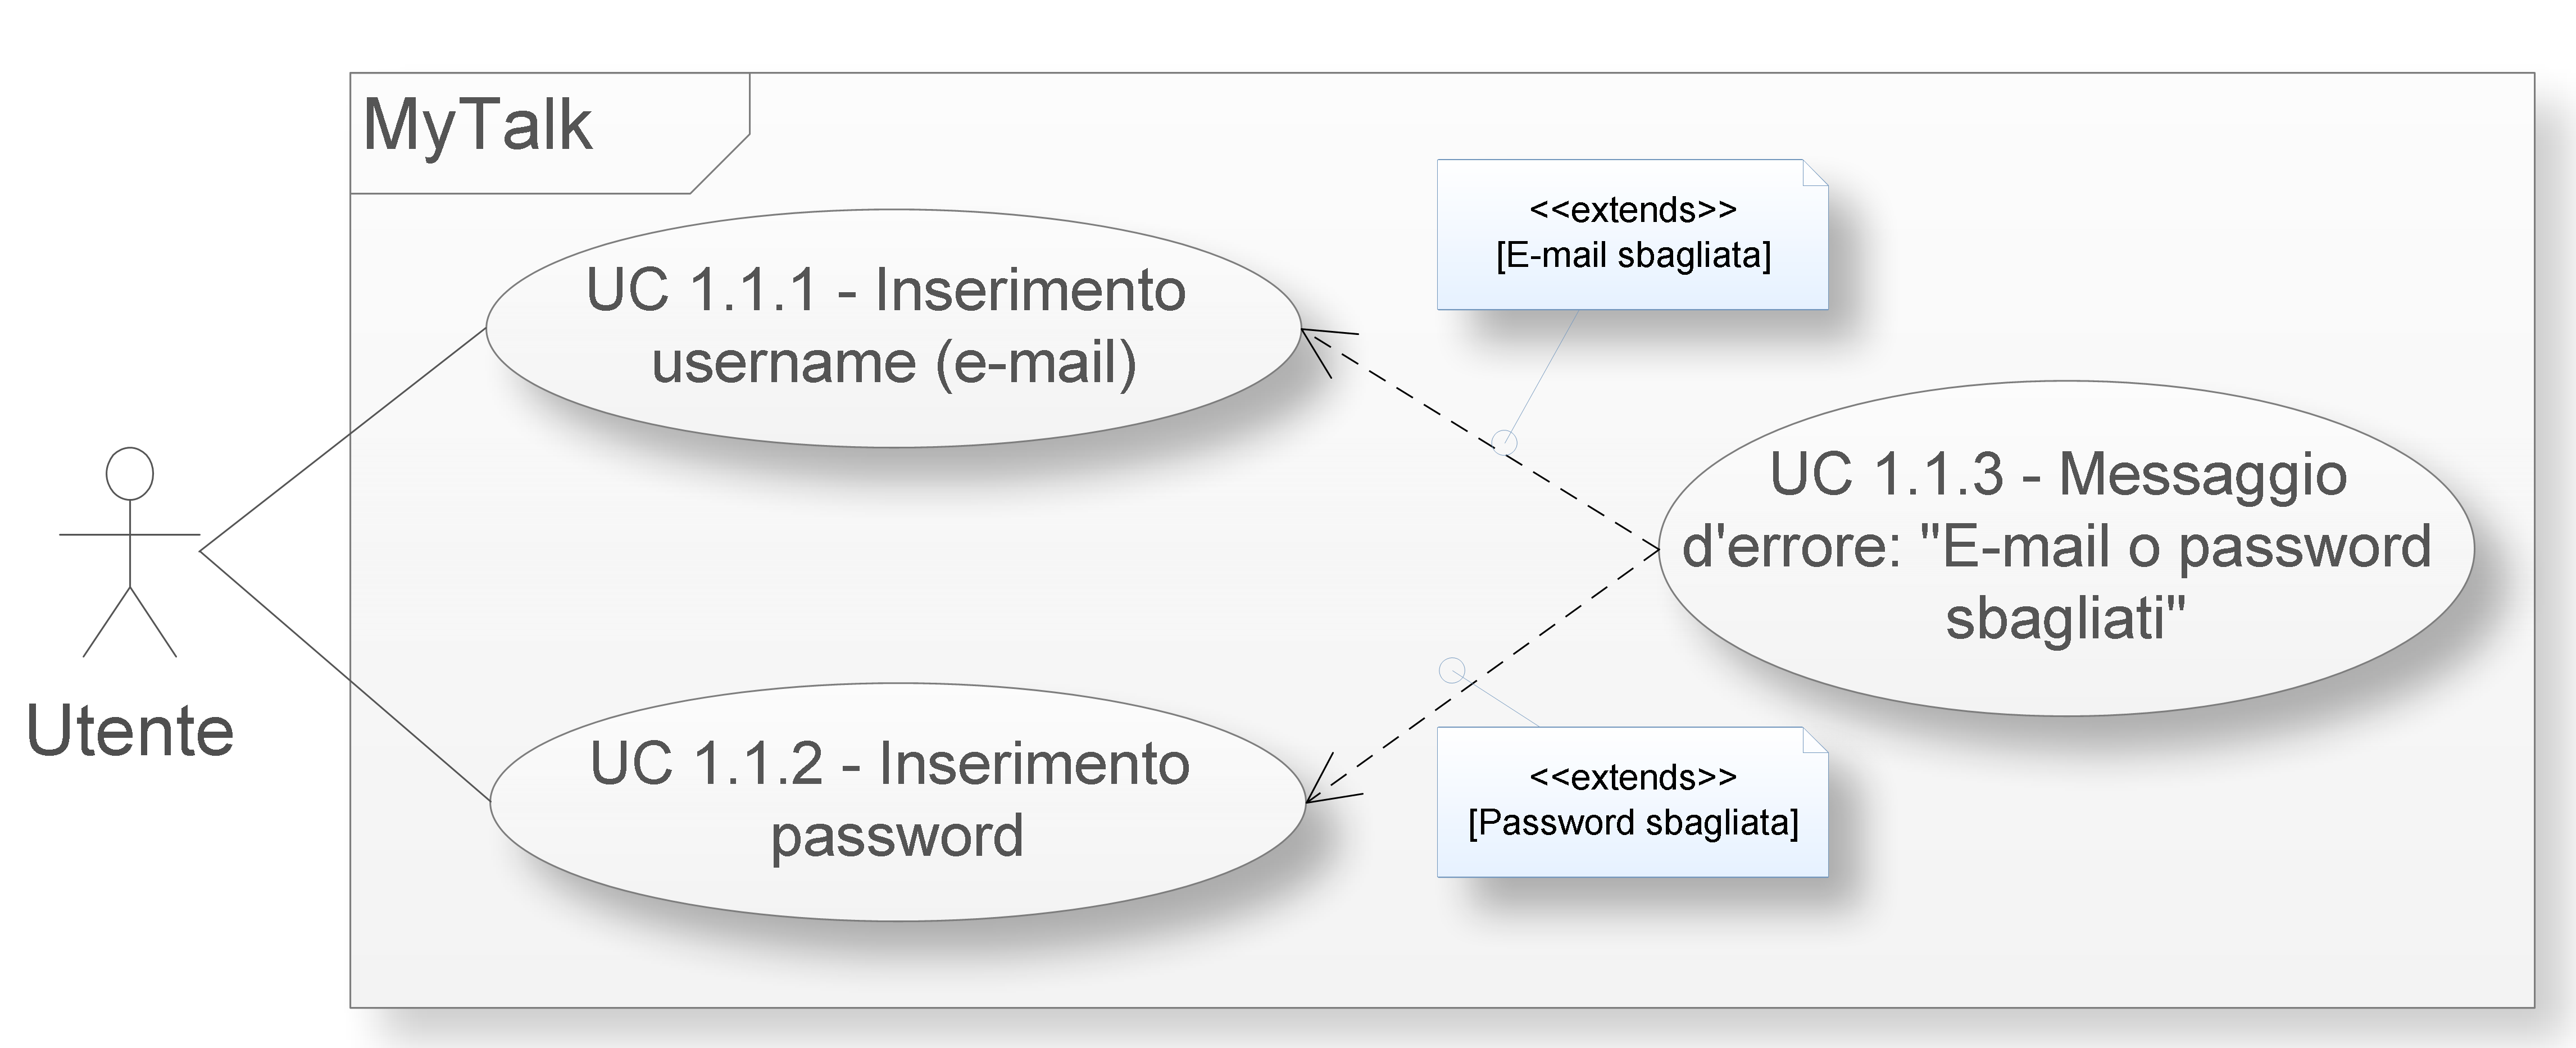
\includegraphics[width=.8\textwidth]{UC1-1}
\caption{}\label{fig:}
\end{center}
\end{figure}
\begin{description}
\item{\scshape\bfseries Attori principali:}Utente.
\item{\scshape\bfseries Scopo e descrizione:} L'utente si autentica per accedere al sistema MyTalk
\item{\scshape\bfseries Precondizione:} L'utente (generico) visualizza la schermata iniziale e il sistema è pronto.
\item{\scshape\bfseries Postcondizione:} L'utente è autenticato nel sistema
\item{\scshape\bfseries Illustrazione scenario principale:} L'utente inserisce username (UC1.1.1) e password (UC1.1.2) corretti e conferma.
\item{\scshape\bfseries Illustrazione scenario alternativo:} L'utente ha inserito dati non corretti: il sistema lo notifica con un errore unico (UC1.1.3) e rimane in attesa di una correzione. (Non vengono visualizzati due errori separati ma un errore unico generico per aumentare la sicurezza).
\end{description}

\subsection{UC1.2: Registrazione}
\begin{figure}[H]
\begin{center}
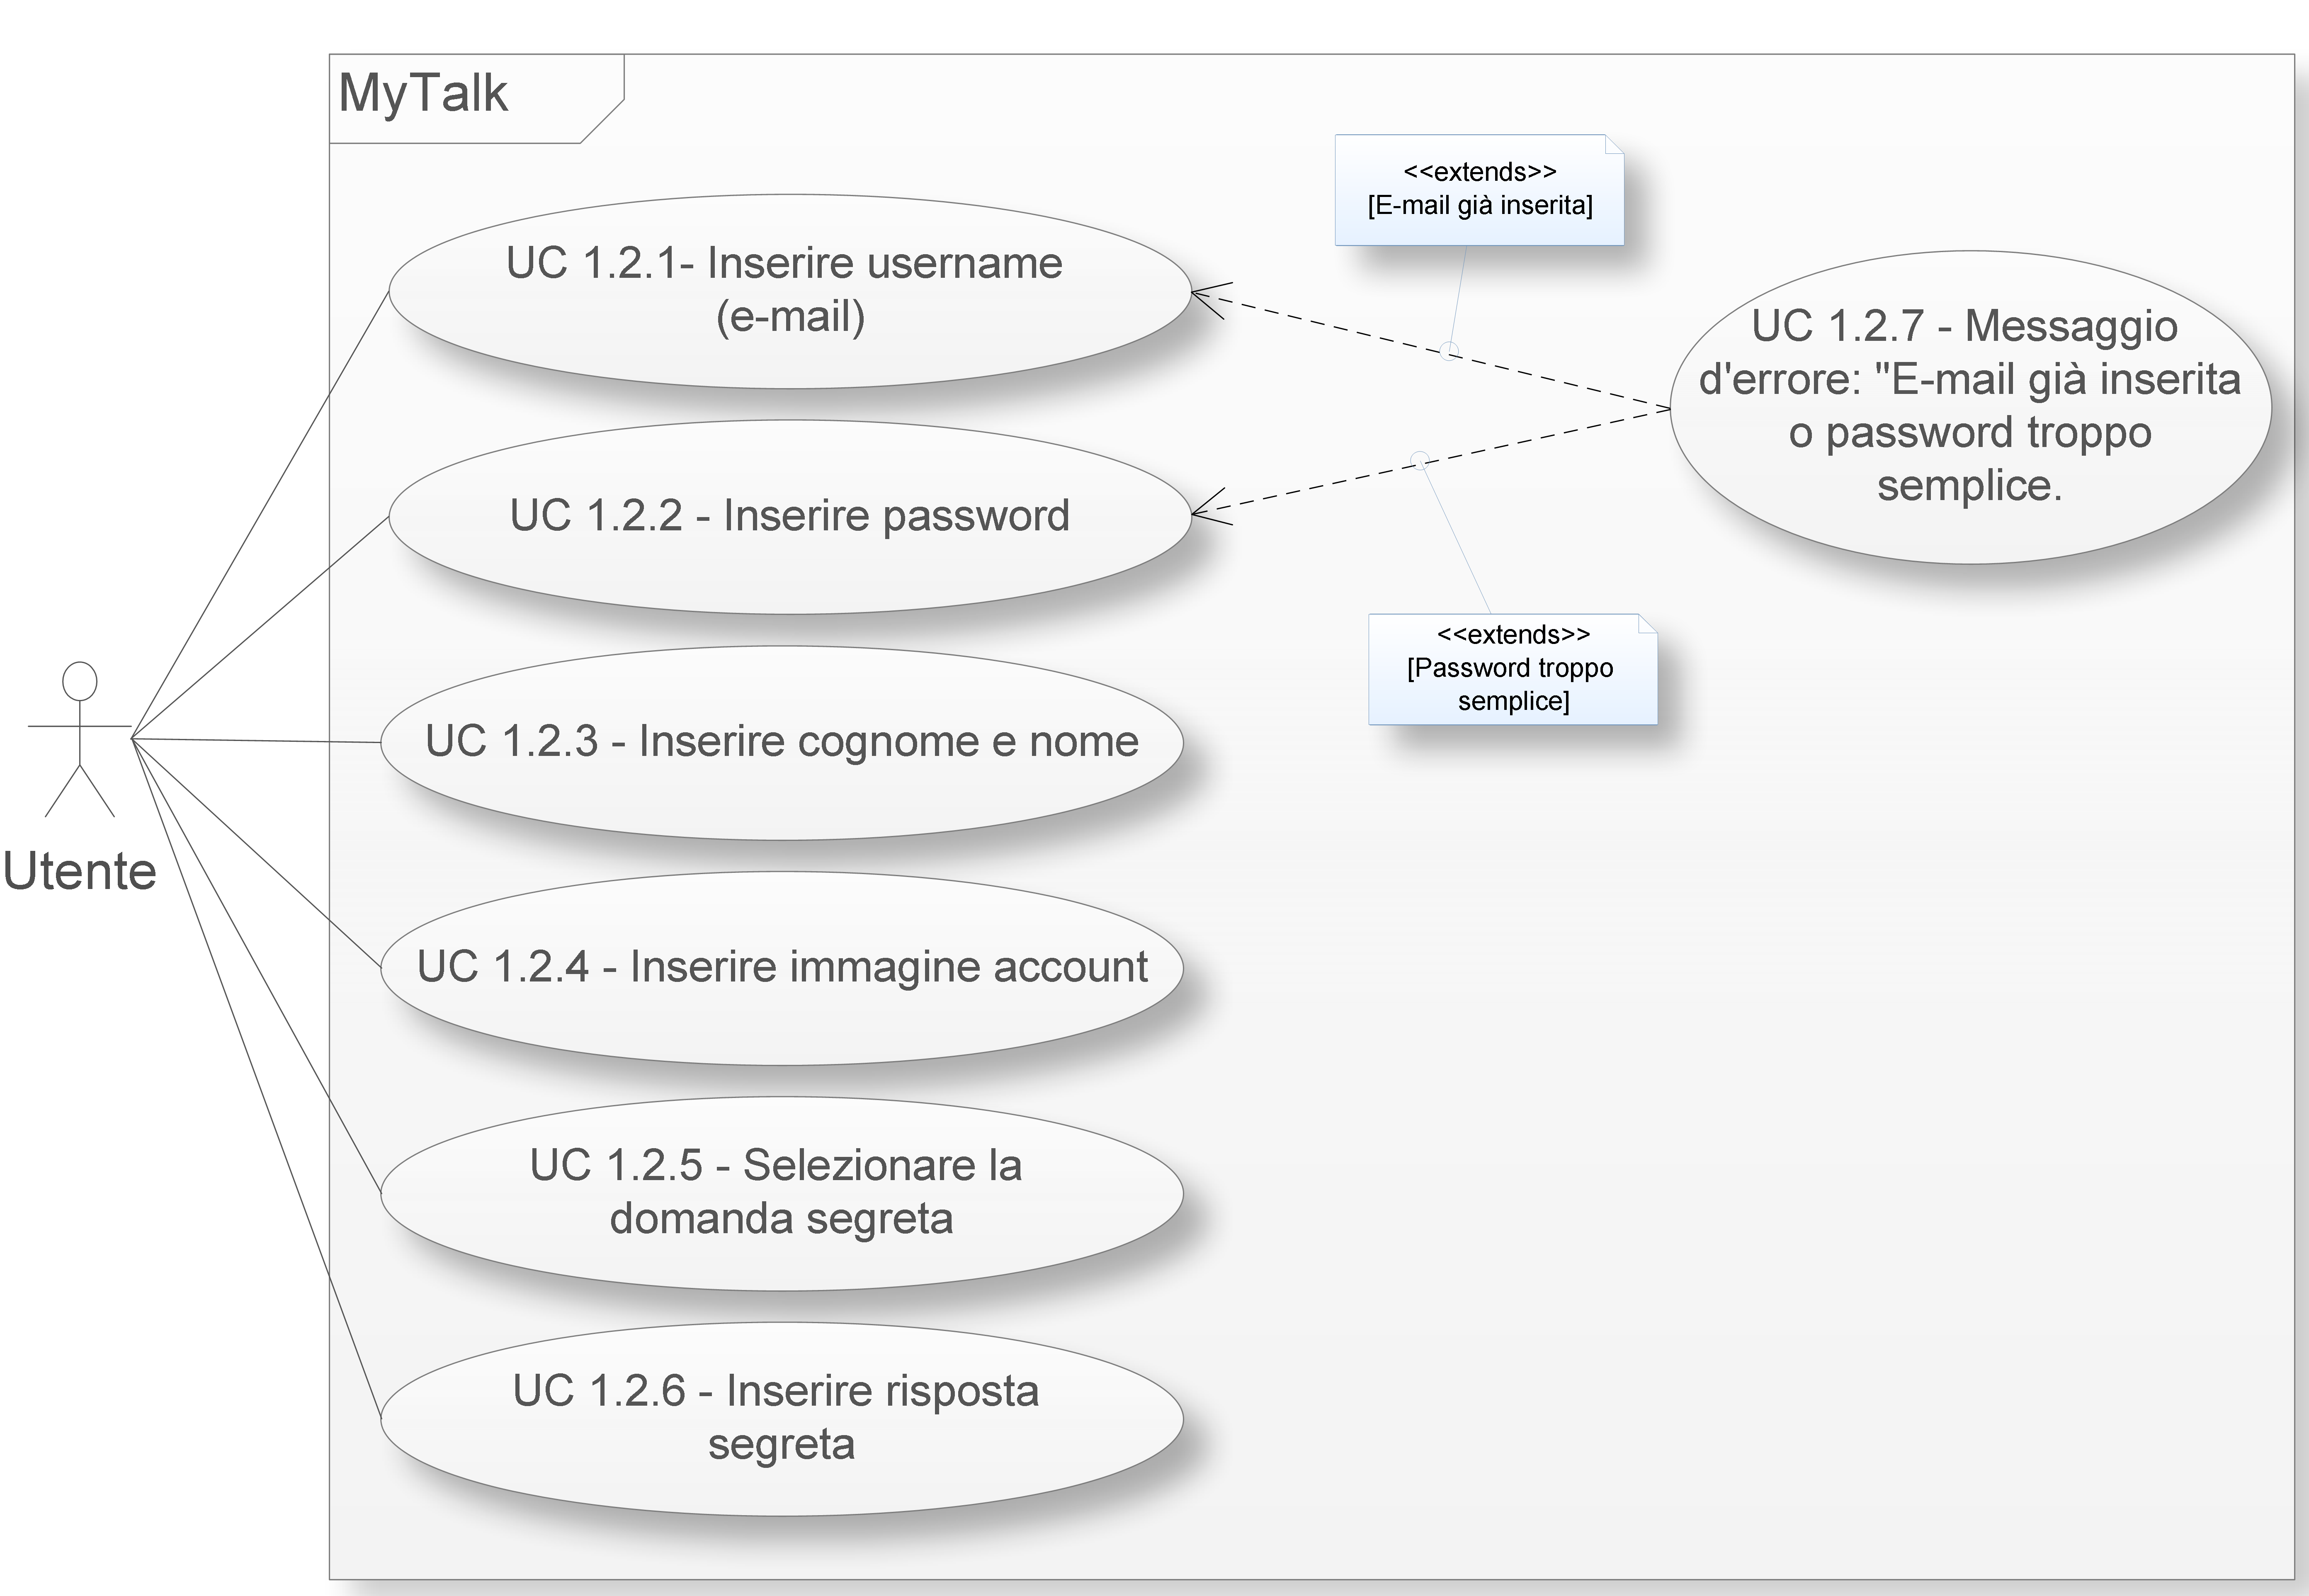
\includegraphics[width=.8\textwidth]{UC1-2}
\caption{}\label{fig:}
\end{center}
\end{figure}
\begin{description}
\item{\scshape\bfseries Attori principali:}Utente.
\item{\scshape\bfseries Scopo e descrizione:} L'utente si registra nel sistema.
\item{\scshape\bfseries Precondizione:} L'utente (generico) visualizza la schermata iniziale e il sistema è pronto.
\item{\scshape\bfseries Postcondizione:} L'utente si è registrato nel sistema MyTalk
\item{\scshape\bfseries Illustrazione scenario principale:} La registrazione di un nuovo account comporta l'inserimento di un indirizzo email come ID utente (UC1.2.1), una password (UC1.2.2), domanda segreta (UC1.2.6) e la relativa risposta (UC1.2.7). Il nome (UC1.2.3), il cognome (UC1.2.4) e un'immagine (UC1.2.5) da associare al proprio profilo possono essere inserite facoltativamente. Per andare a buon fine la procedura di registrazione richiede che la password prescelta assicuri un sufficiente livello di complessità e prevede altresì la selezione della domanda segreta (e della relativa risposta) necessarie al recupero della password in caso di smarrimento, nonché la validazione dell''indirizzo email al fine di verificare che l''utente ne sia effettivamente in possesso.
\item{\scshape\bfseries Illustrazione scenario alternativo:} Il sistema può fallire per via dell'inserimento di dati non corretti. Il sistema mostra un errore relativo all'username (UC1.2.8) oppure alla password (UC1.2.9)
\end{description}

\subsection{UC1.3: Recupero della password}
\begin{figure}[H]
\begin{center}
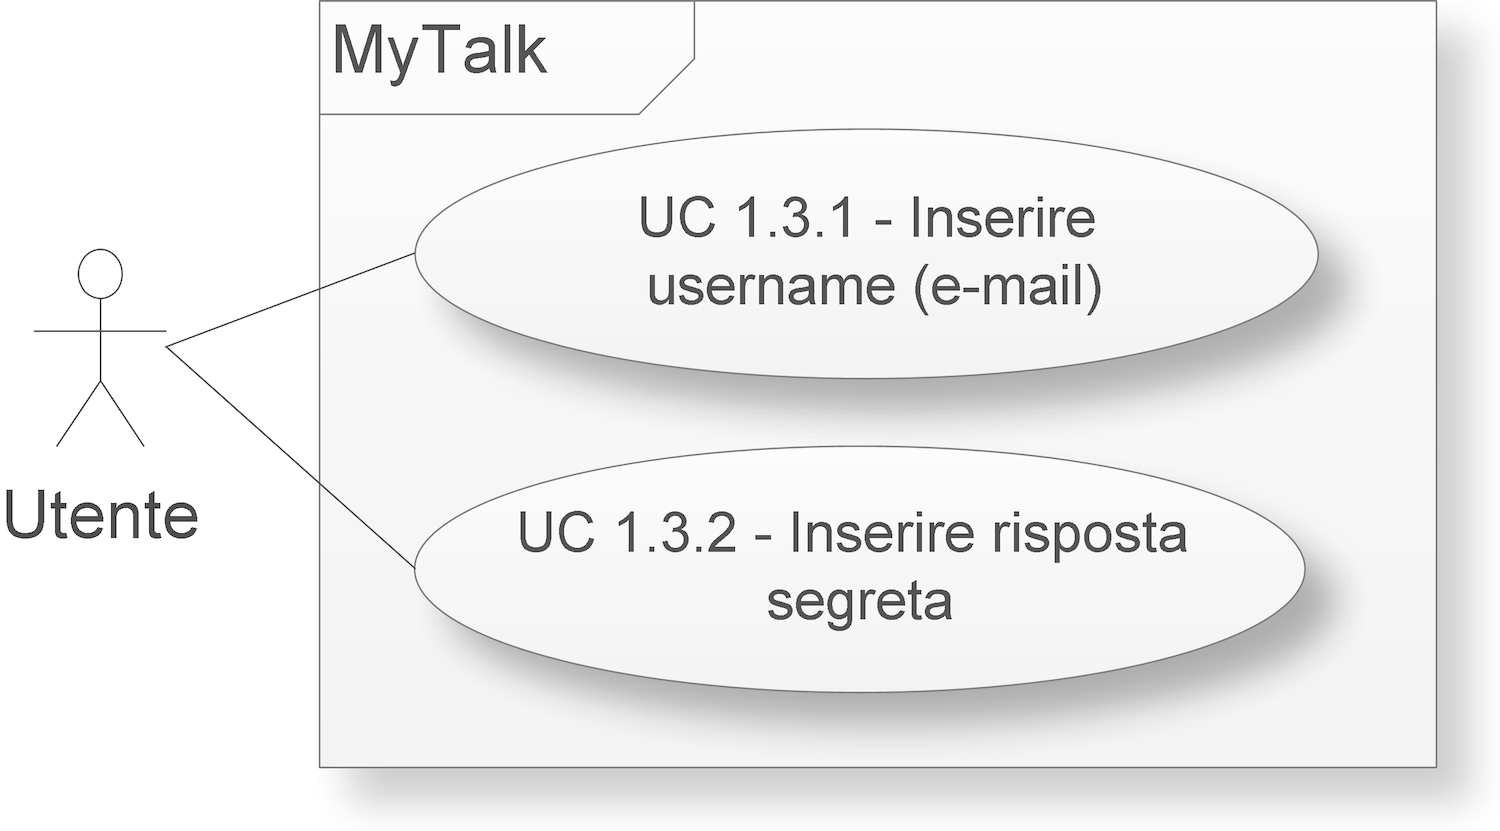
\includegraphics[width=.8\textwidth]{UC1-3}
\caption{}\label{fig:}
\end{center}
\end{figure}
\begin{description}
\item{\scshape\bfseries Attori principali:}Utente.
\item{\scshape\bfseries Scopo e descrizione:} L'utente desidera recuperare la password smarrita.
\item{\scshape\bfseries Precondizione:} L'utente (generico) visualizza la schermata iniziale e il sistema è pronto.
\item{\scshape\bfseries Postcondizione:} L'utente riceve per e-mail la password dimenticata.
\item{\scshape\bfseries Illustrazione scenario principale:} Si avvia la procedura di recupero della password: l'utente deve inserire l'e-mail (UC1.3.1) e la risposta alla domanda segreta (UC1.3.2). A questo segue l'invio della password all'indirizzo email indicato in fase di registrazione.
\item{\scshape\bfseries Illustrazione scenario alternativo:} Il sistema può fallire per via dell'inserimento di dati non corretti. Il sistema evidenzia gli errori e rimane in attesa della correzione.
\end{description}

\subsection{UC2: Home screen dell'applicativo}
\begin{figure}[H]
\begin{center}
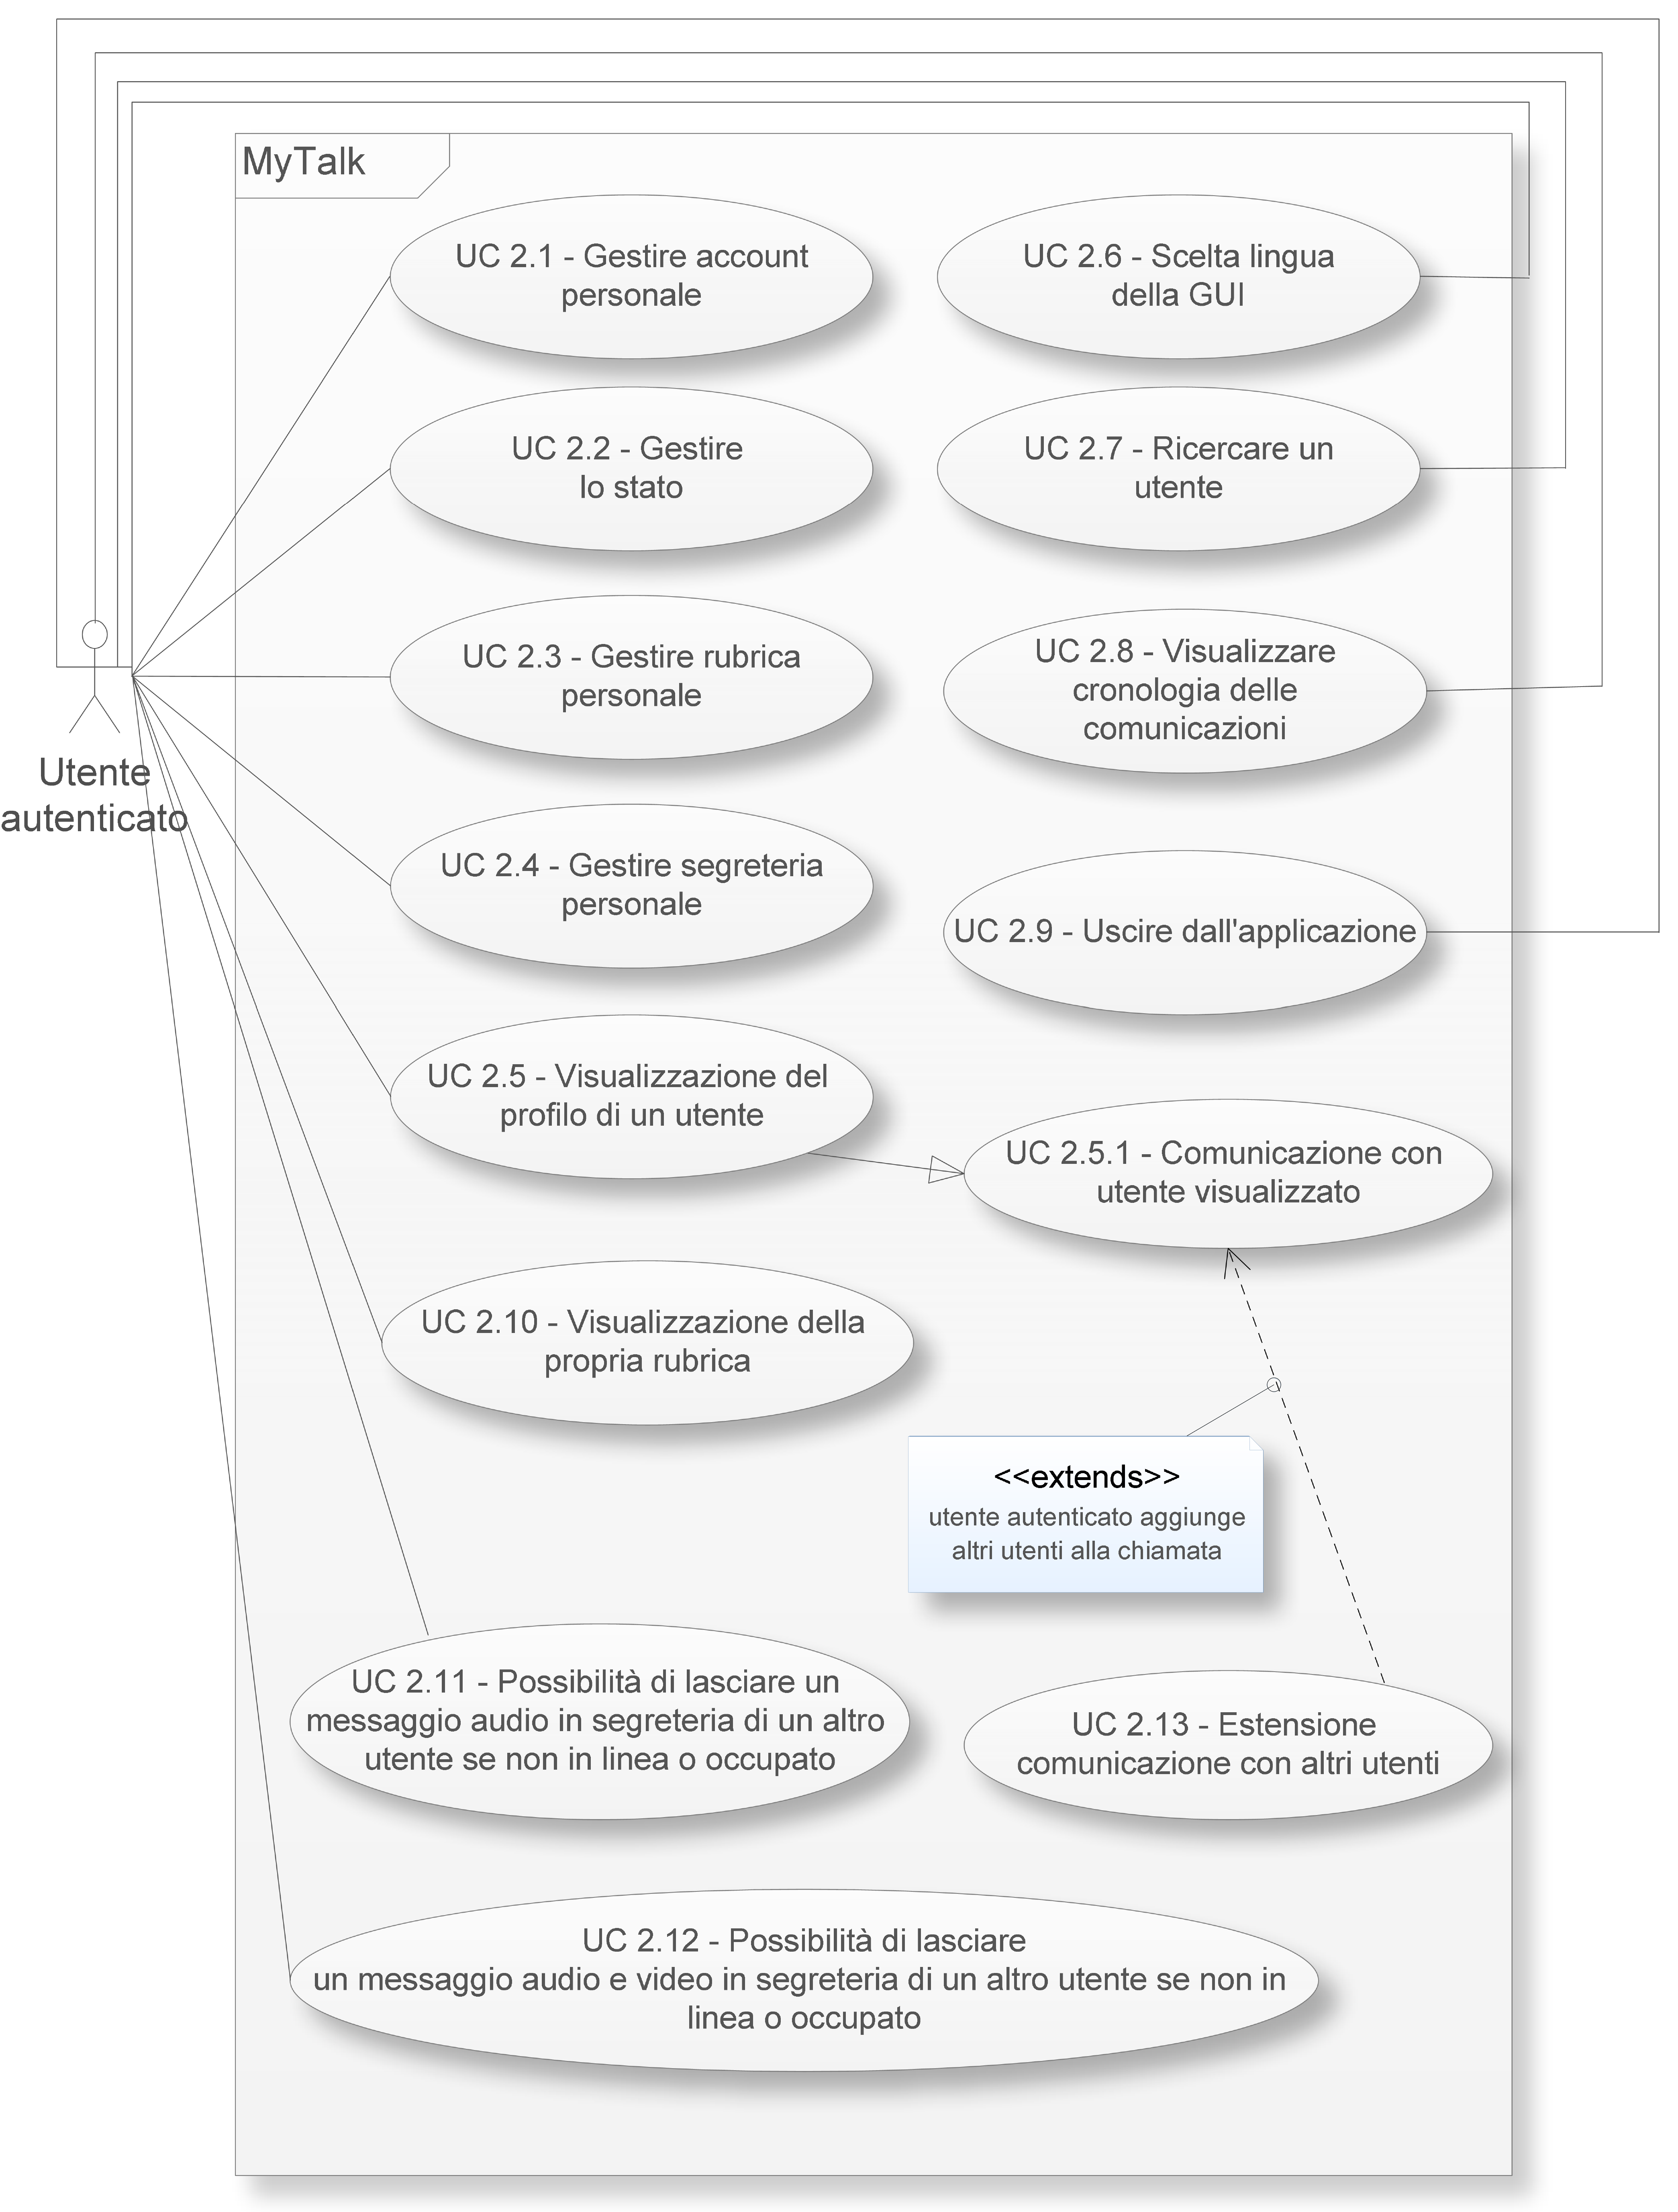
\includegraphics[width=.8\textwidth]{UC2}
\caption{}\label{fig:}
\end{center}
\end{figure}
\begin{description}
\item{\scshape\bfseries Attori principali:}Utente autenticato.
\item{\scshape\bfseries Scopo e descrizione:} Funzionalità generali offerte all'utente autenticato e presenti nella Home screen dell'applicativo.
\item{\scshape\bfseries Precondizione:} L'utente ha effettuato il login ed è autenticato nel sistema.
\item{\scshape\bfseries Postcondizione:} L'utente ha eseguito una delle funzioni proposte.
\item{\scshape\bfseries Illustrazione scenario principale:} L'utente dopo aver eseguito il login al sistema, si trova nella Home dell'applicativo. Qui può svolgere una delle seguenti operazioni: gestire il proprio account (UC2.1), scegliere la lingua della GUI (UC2.6), gestire lo stato (UC2.2), eseguire delle ricerche di utenti (UC2.7), gestire la propria rubrica (UC2.3), lasciare un messaggio nella segreteria di un utente se esso non è in linea o è occupato (UC2.11 - UC2.12), gestire la propria segreteria (UC2.4), visualizzare la cronologia delle comunicazioni (UC2.8), visualizzare la propria rubrica (UC2.10) e visualizzare il profilo di un utente (UC2.5) dopo averlo selezionato da una lista. Infine l'utente ha la possibilità di chiudere l'applicativo (UC2.9).
\item{\scshape\bfseries Illustrazione scenario alternativo:} L'utente, se ha già avviato una connessione con un altro utente, può estenderla con altri (UC2.12).
\end{description}

\subsection{UC2.1: Gestione account}
\begin{figure}[H]
\begin{center}
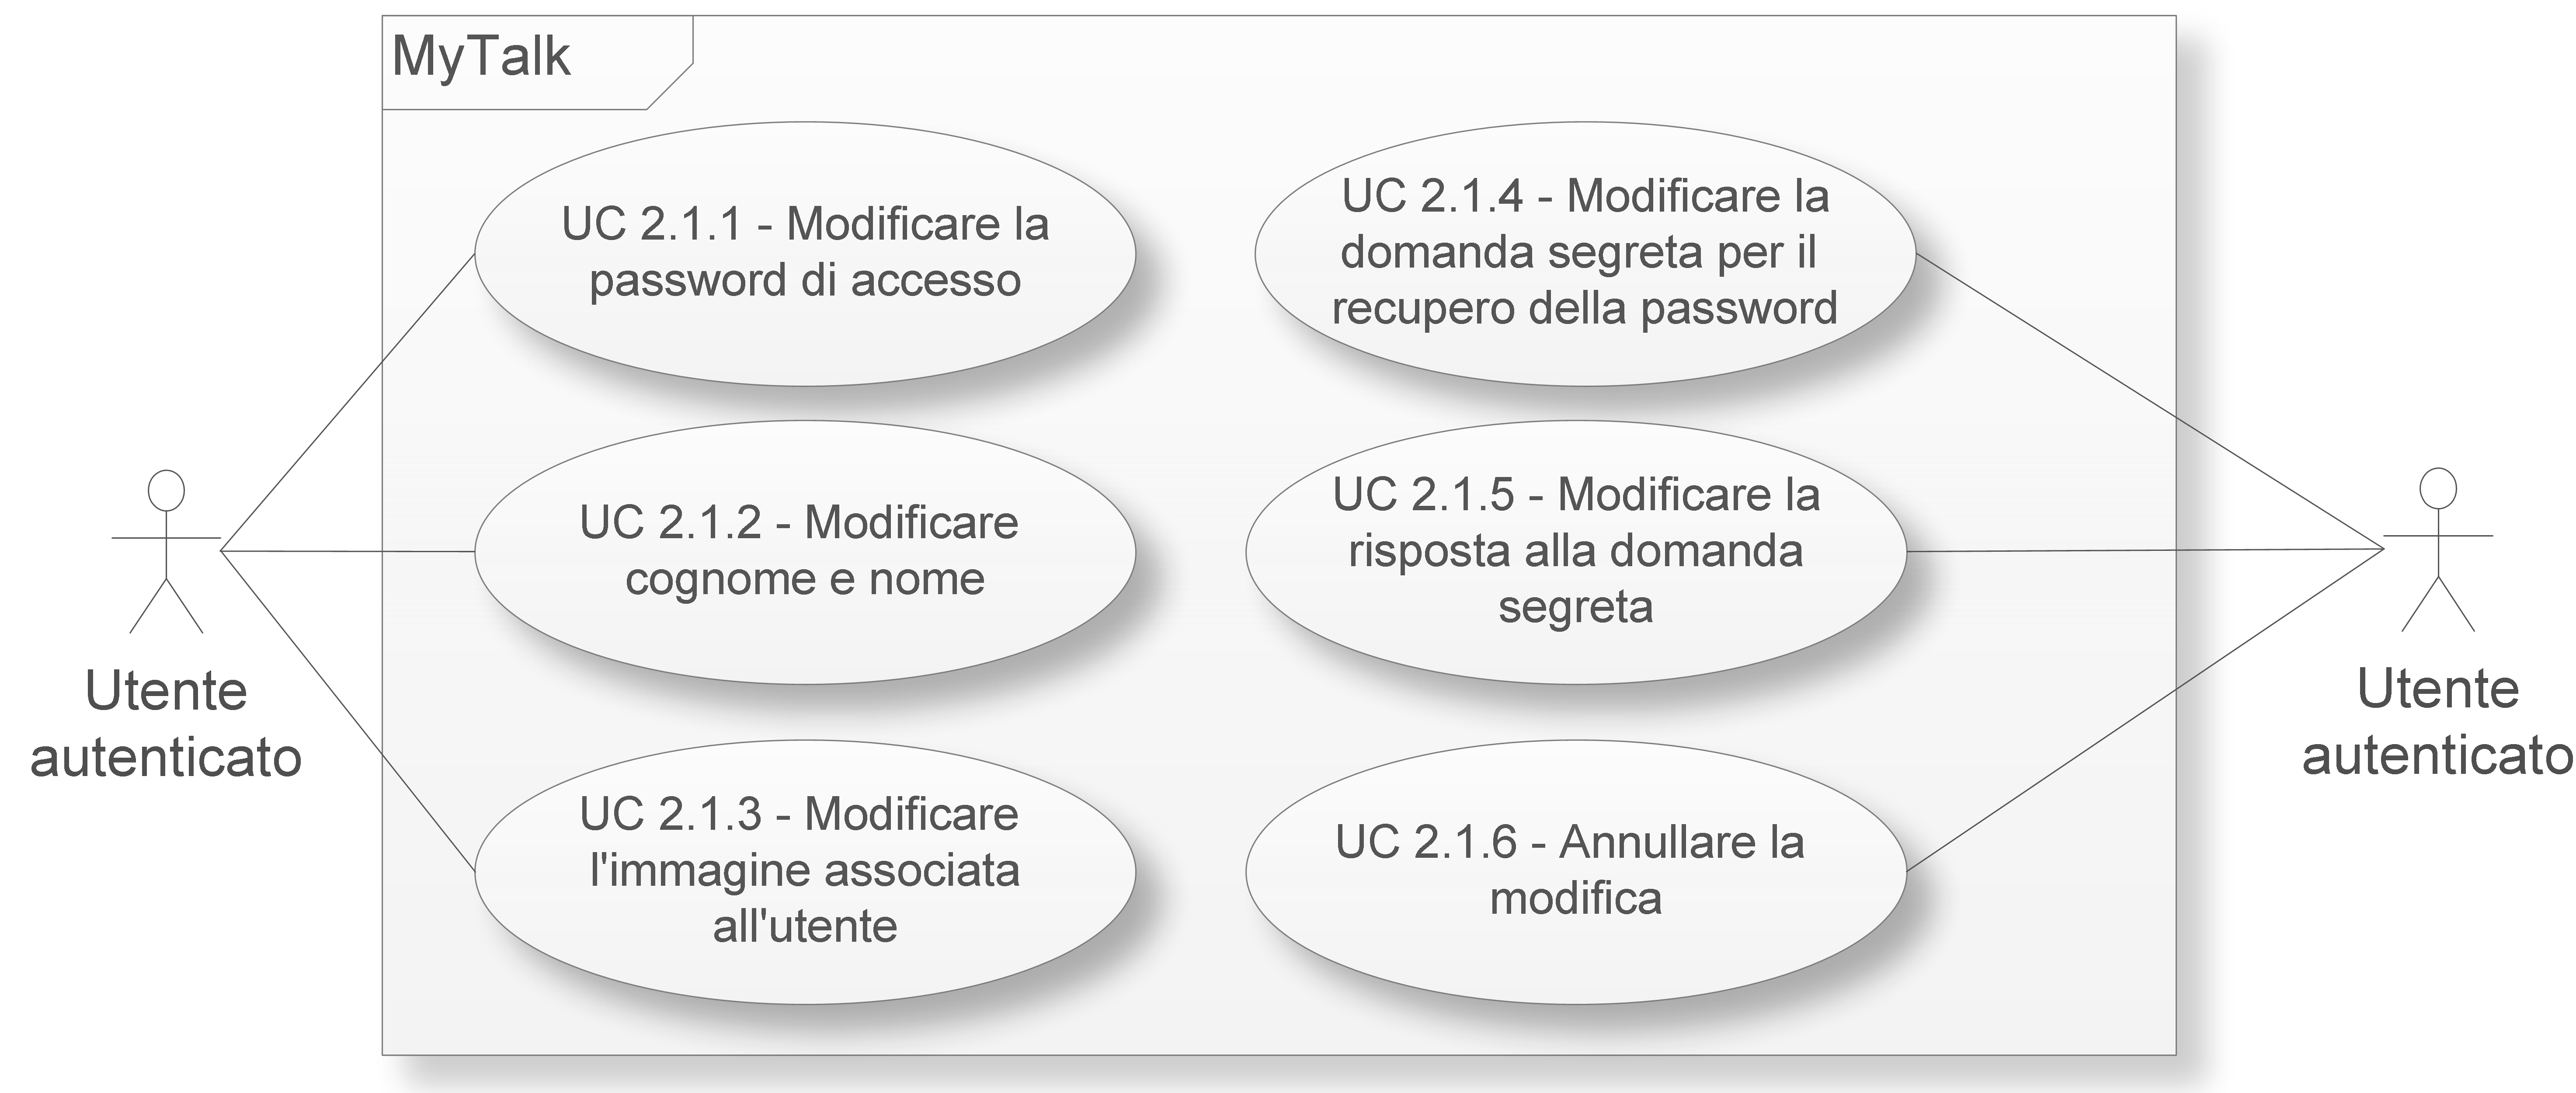
\includegraphics[width=.8\textwidth]{UC2-1}
\caption{}\label{fig:}
\end{center}
\end{figure}
\begin{description}
\item{\scshape\bfseries Attori principali:}Utente autenticato.
\item{\scshape\bfseries Scopo e descrizione:} un utente autenticato, ha la possibilità di modificare i propri dati personali, inseriti durante la sua registrazione, così da rimediare ad eventuali errori.
\item{\scshape\bfseries Precondizione:} l'utente corrente e' registrato nel sistema, ed ha effettuato il login.
\item{\scshape\bfseries Postcondizione:} i dati dell'utente sono stati aggiornati con i valori da lui inseriti.
\item{\scshape\bfseries Illustrazione scenario principale:} L'utente visualizza i valori correnti dei dati che lo riguardano e può apportare
le modifiche che ritiene necessarie. I dati che può modificare sono la password (UC2.1.1), il nome (UC2.1.2), il cognome (UC2.1.6), l'immagine profilo (UC2.1.3), la domanda segreta (UC2.1.4), la risposta alla domanda segreta (UC2.1.5). A questo punto può salvare le modifiche (UC2.1.8).
\item{\scshape\bfseries Illustrazione scenario alternativo:} Prima del salvataggio (UC2.1.8) l'utente può annullare l'operazione (UC2.1.7) tornando così alla schermata principale senza aver effettuato nessuna modifica.
\end{description}

\subsection{UC2.2: Gestire lo stato}
\begin{figure}[H]
\begin{center}
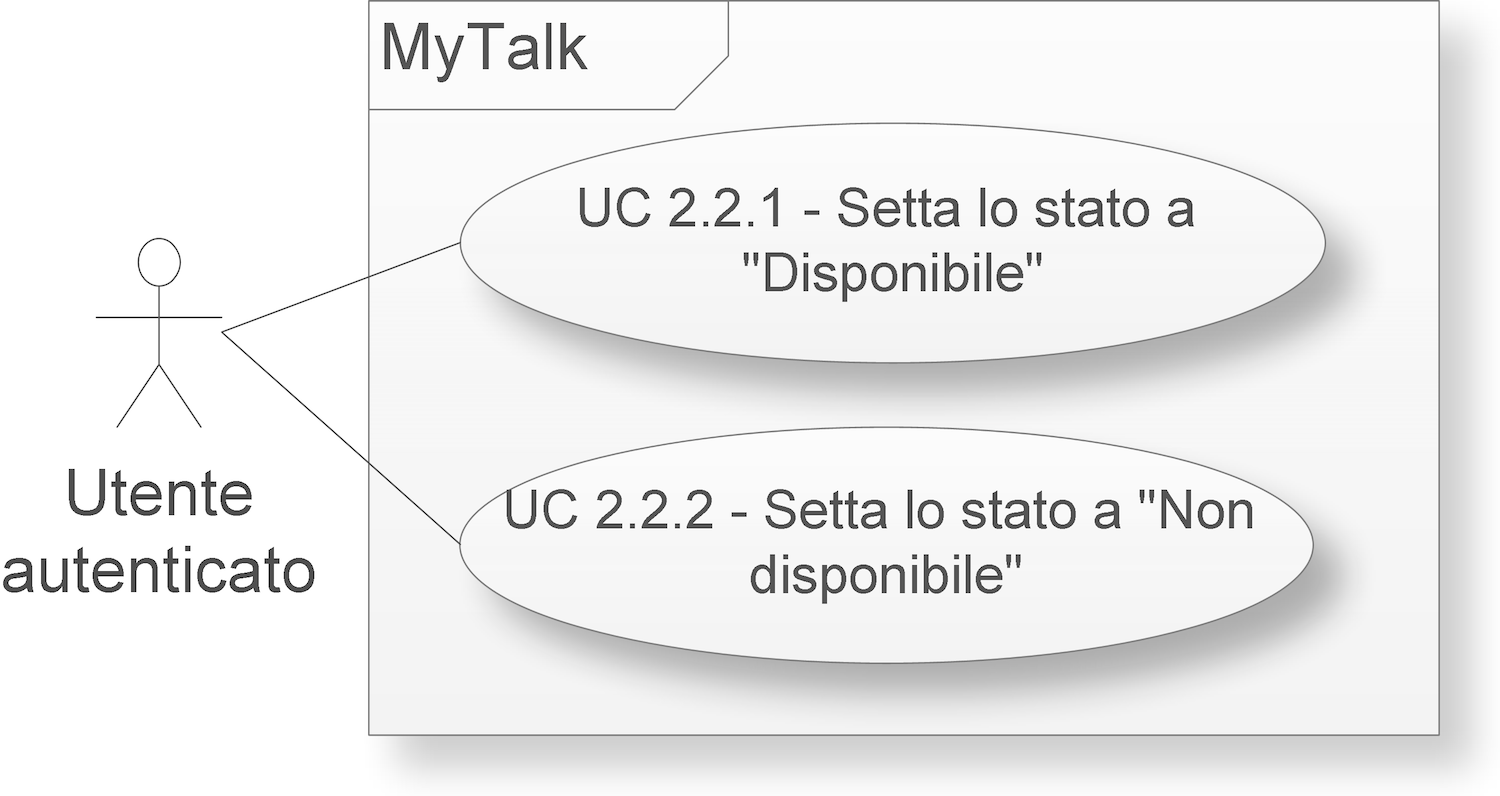
\includegraphics[width=.8\textwidth]{UC2-2}
\caption{}\label{fig:}
\end{center}
\end{figure}
\begin{description}
\item{\scshape\bfseries Attori principali:}Utente autenticato.
\item{\scshape\bfseries Scopo e descrizione:} L'utente potrà comunicare agli altri utenti la sua disponibilità o meno a comunicare, aggiornando il proprio stato.
\item{\scshape\bfseries Precondizione:} L'utente è registrato nel sistema ed ha eseguito l'accesso senza errori.
\item{\scshape\bfseries Postcondizione:} L'utente ha modificato il proprio stato.
\item{\scshape\bfseries Illustrazione scenario principale:} L'utente potrà scegliere di cambiare il proprio stato corrente. Gli stati tra cui può scegliere sono:disponibile (UC2.2.1)  e non disponibile (UC2.2.2).
\end{description}

\subsection{UC2.3: Gestione della rubrica}
\begin{figure}[H]
\begin{center}
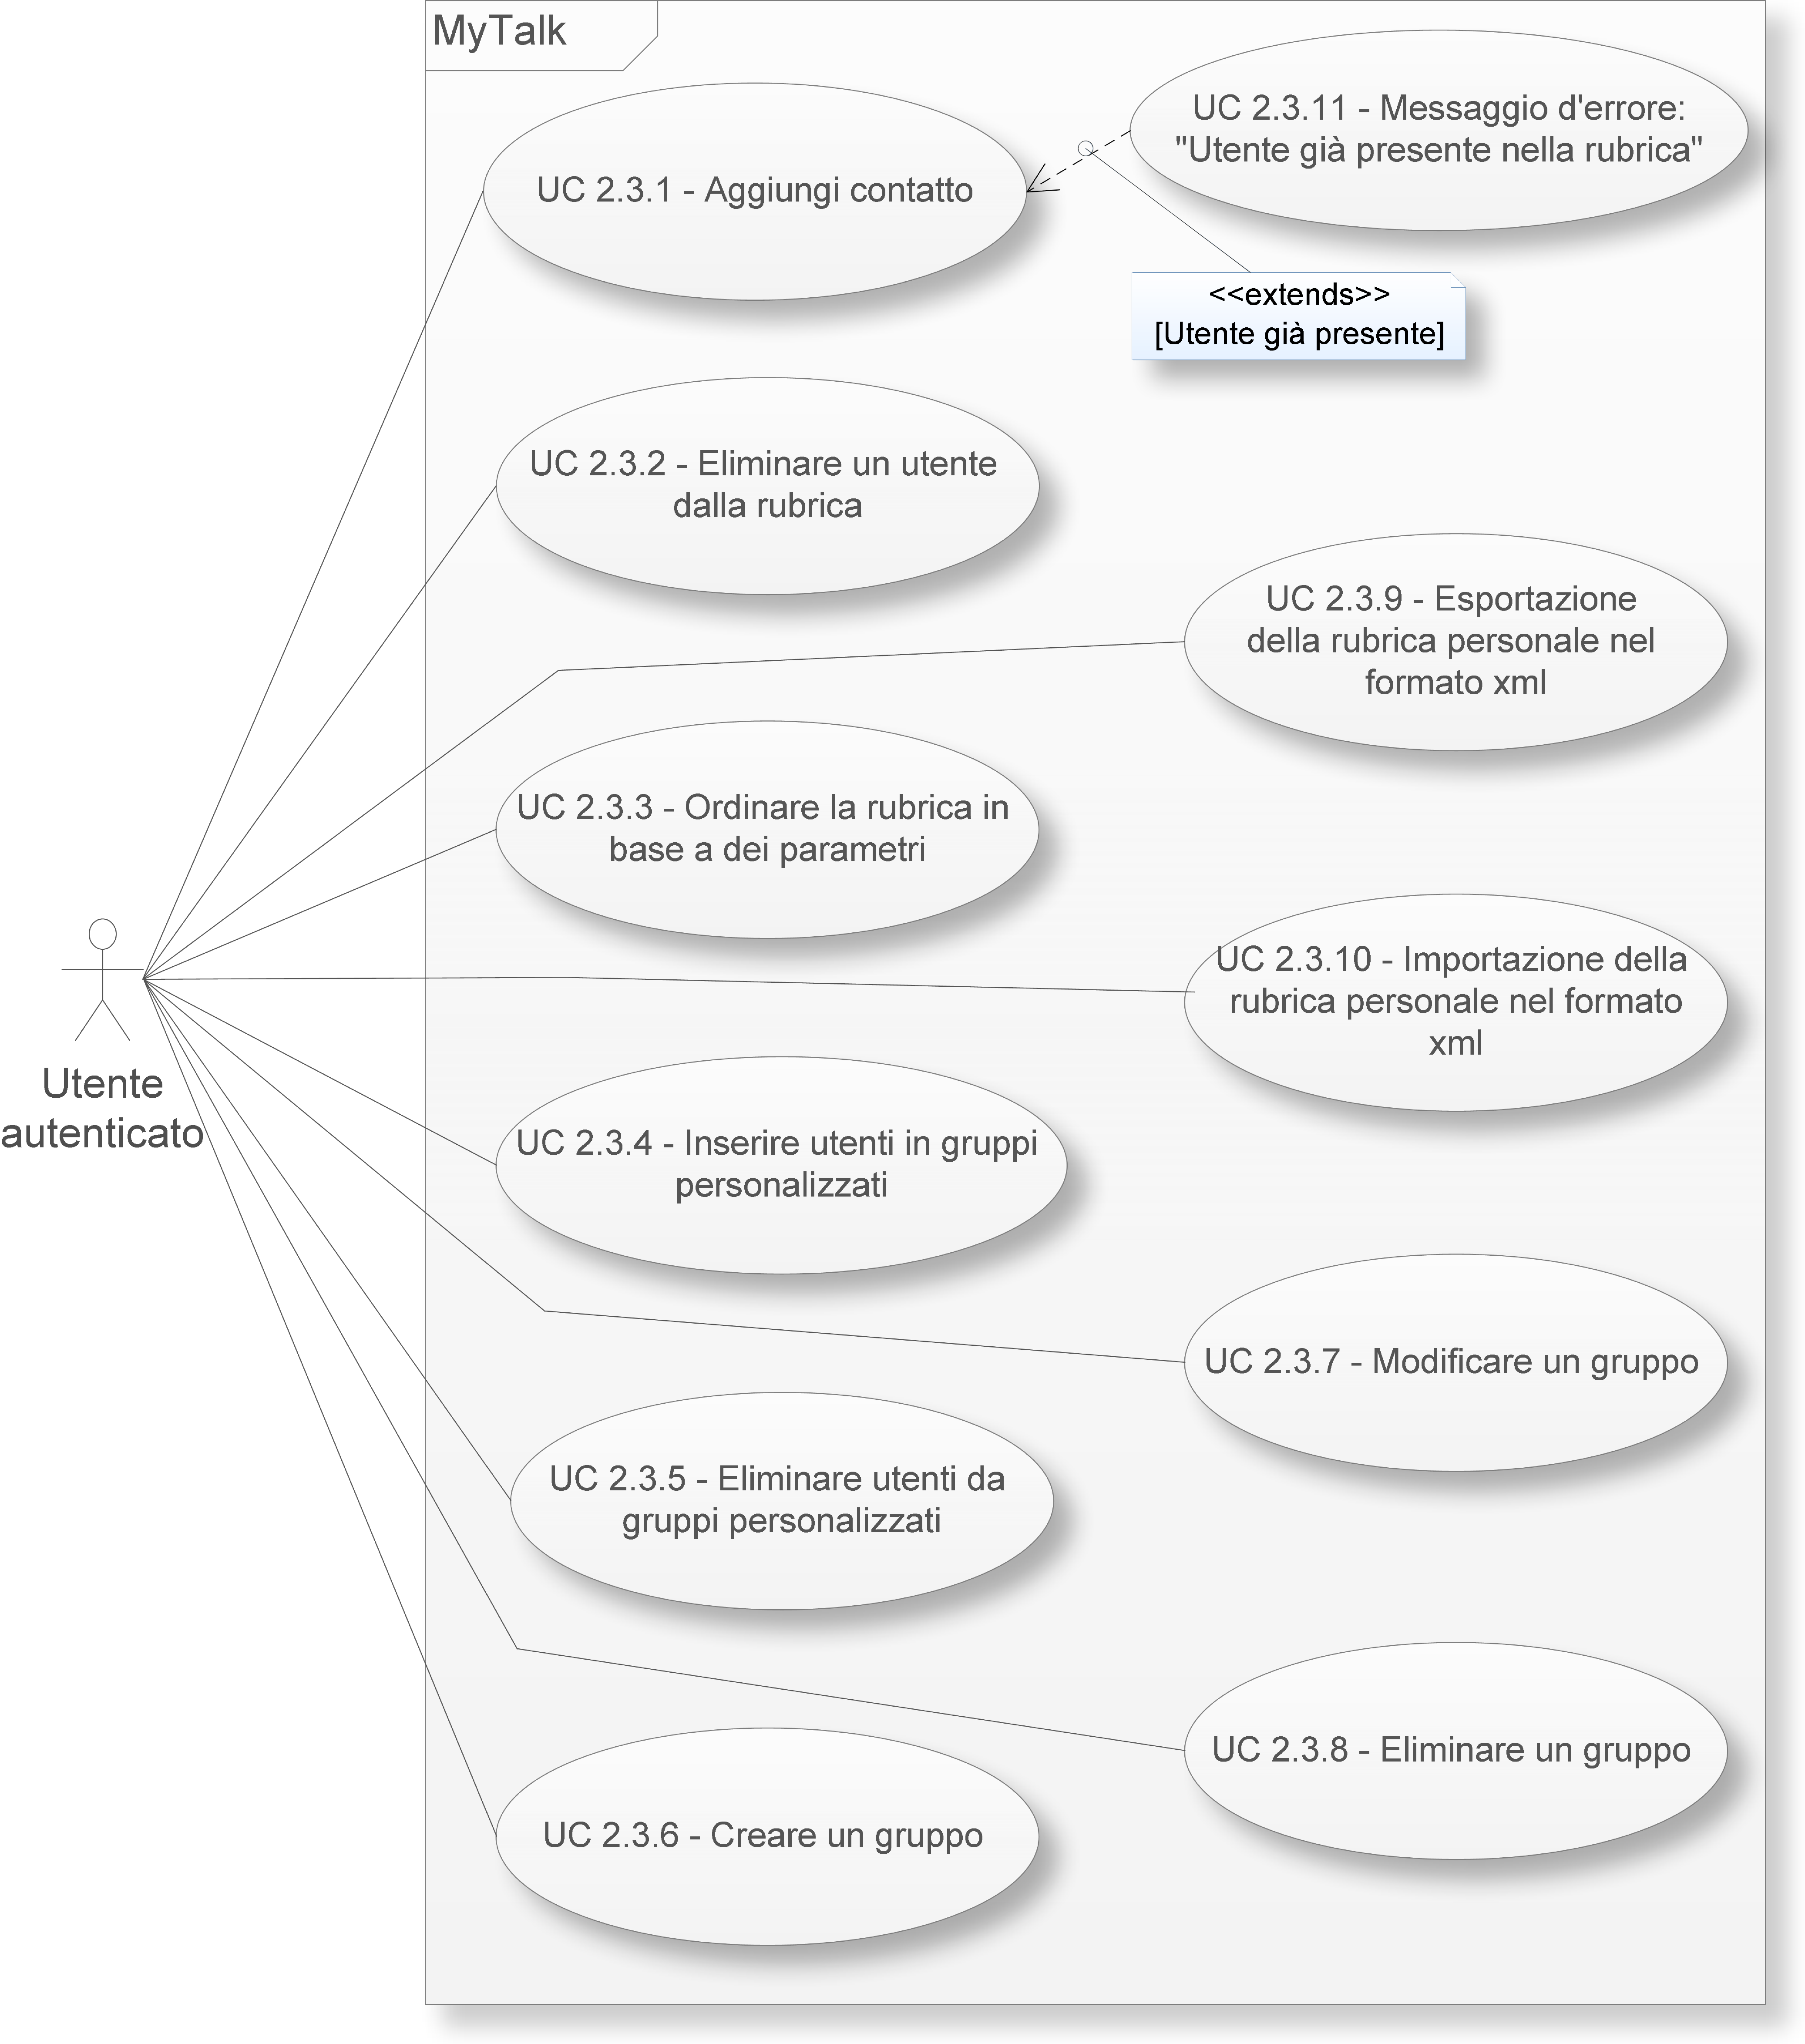
\includegraphics[width=.8\textwidth]{UC2-3}
\caption{}\label{fig:}
\end{center}
\end{figure}
\begin{description}
\item{\scshape\bfseries Attori principali:}Utente autenticato.
\item{\scshape\bfseries Scopo e descrizione:} L'utente può visualizzare ed organizzare la rubrica dei propri contatti personali sulla base della lista degli utenti che si sono registrati, oppure importando i contati da un file esterno.
\item{\scshape\bfseries Precondizione:} L'utente ha effettuato la procedura di login ed è quindi autenticato.
\item{\scshape\bfseries Postcondizione:} Se l'utente ha attuato delle modifiche, queste sono state salvate. Altrimenti non ci sono state modifiche sui dati inerenti la rubrica.
\item{\scshape\bfseries Illustrazione scenario principale:} L'utente visualizza la propria rubrica divisa in gruppi. Può quindi scegliere una delle seguenti opzioni: aggiunge un contatto alla rubrica tramite ricerca (UC2.3.1), aggiunge un contatto in gruppi personalizzati (UC2.3.4), crea un nuovo gruppo (UC2.3.6); elimina un gruppo (UC2.3.8), aggiunge ed eliminare un contatto alla rubrica in un gruppo scelto tra quelli già creati (UC2.3.4 - UC2.3.5), elimina un contatto dalla propria rubrica (UC2.3.2), esporta i contatti presenti nella propria rubrica (UC2.3.9) e importa dei contatti prelevati da un file XML (UC2.3.10).
Inoltre potrà ordinare la rubrica in base a dei parametri (UC2.3.3).
\item{\scshape\bfseries Illustrazione scenario alternativo:} Se la ricerca del contatto da esito negativo viene riportato un errore (UC2.3.1.3).
\item{\scshape\bfseries Illustrazione scenario alternativo:} Se il contatto selezionato per l'inserimento nella rubrica, è già presente nella rubrica, allora compare un messaggio d'errore (UC2.3.1.3) che avvisa l'utente dell'impossibilità di aggiungere il contatto. (Non vengono visualizzati due errori separati ma un errore unico).
\end{description}

\subsection{UC2.4: Gestire segreteria personale}
\begin{figure}[H]
\begin{center}
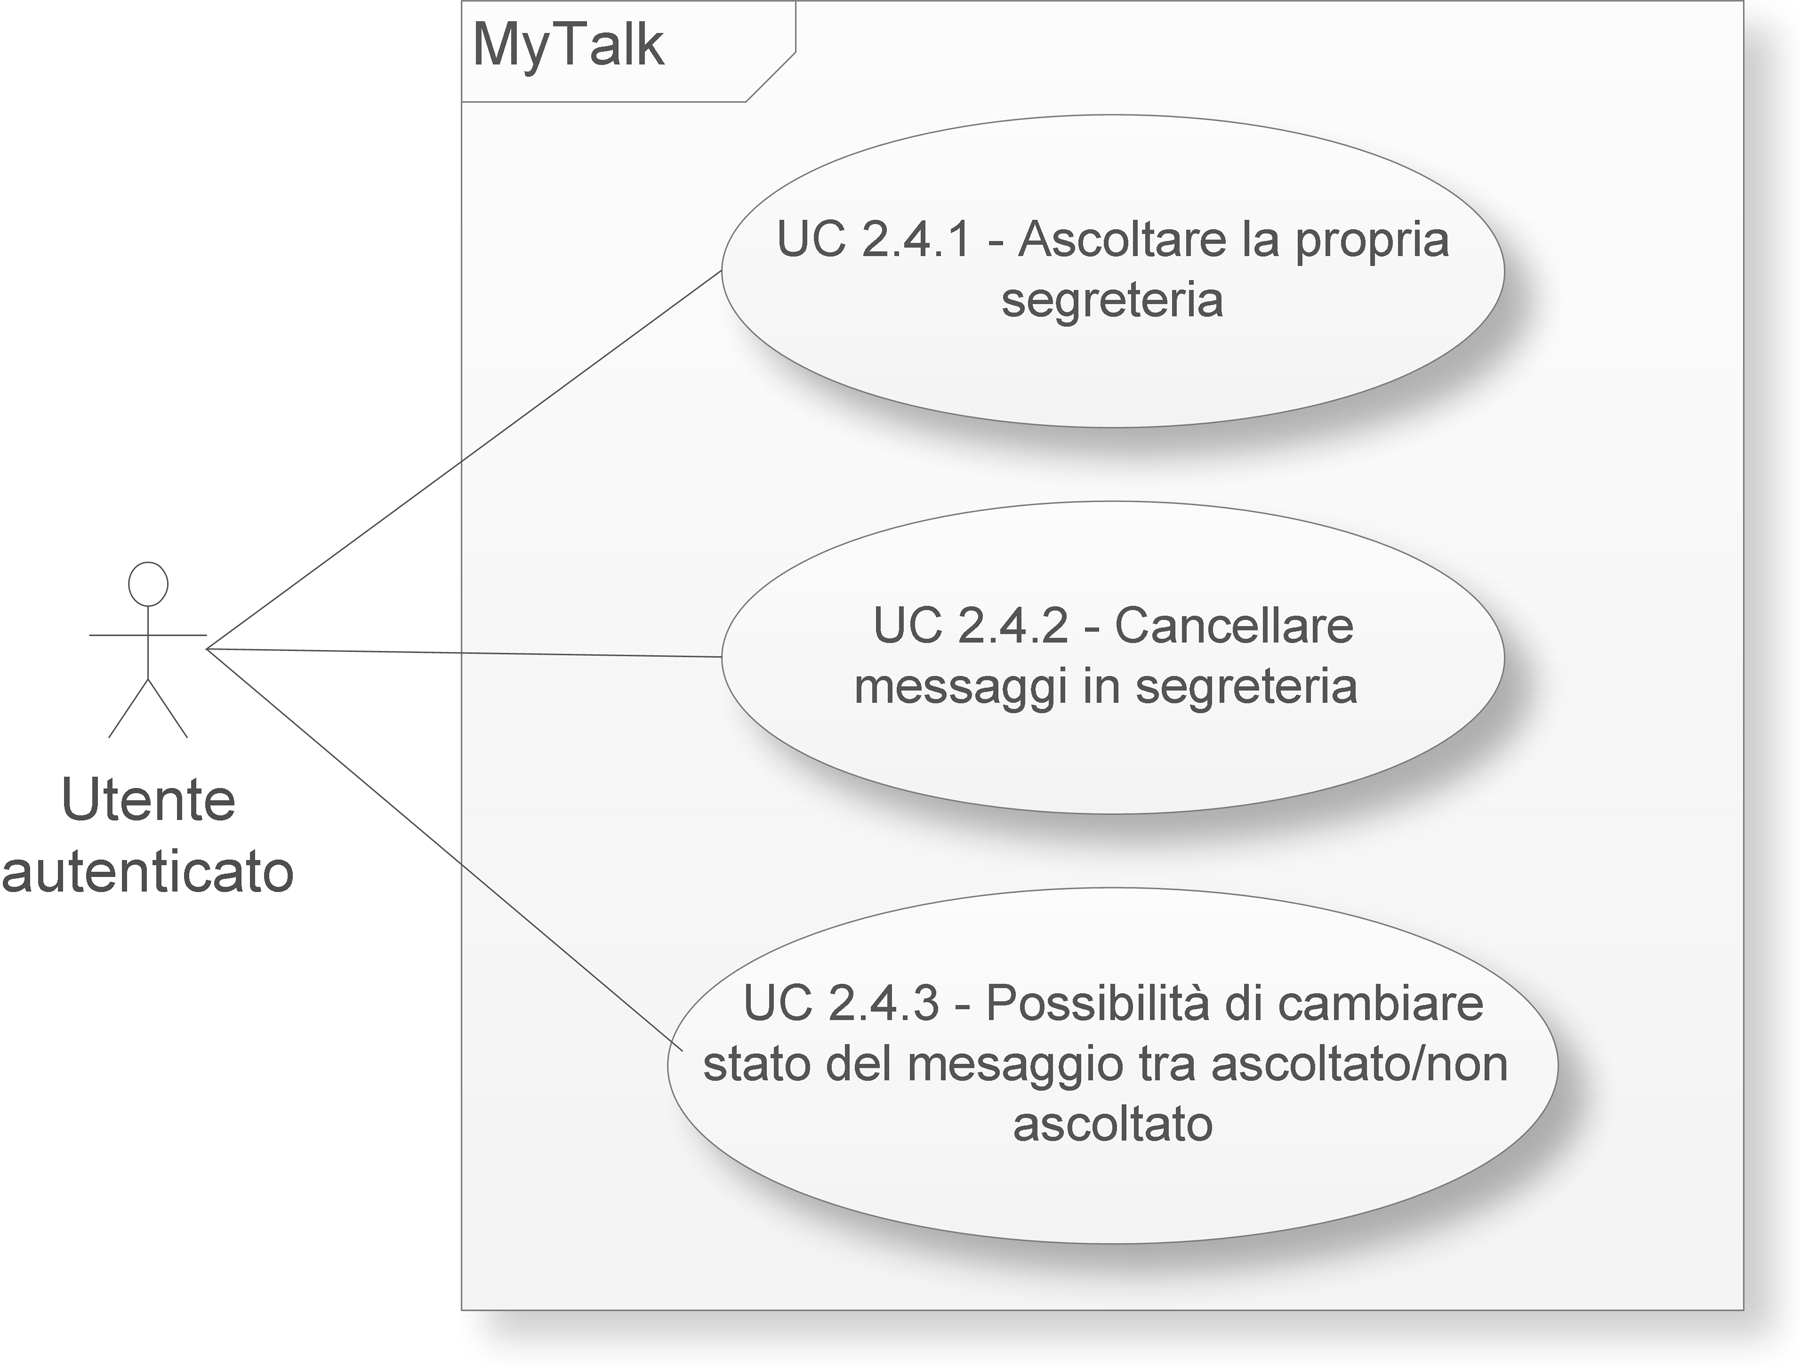
\includegraphics[width=.8\textwidth]{UC2-4}
\caption{}\label{fig:}
\end{center}
\end{figure}
\begin{description}
\item{\scshape\bfseries Attori principali:}Utente autenticato.
\item{\scshape\bfseries Scopo e descrizione:} L'utente ha a disposizione una segreteria personale che può gestire.
\item{\scshape\bfseries Precondizione:} L'utente ha effettuato la procedura di login ed è quindi autenticato.
\item{\scshape\bfseries Postcondizione:} Il sistema ha eseguito con successo le operazioni richieste dall'utente.
\item{\scshape\bfseries Illustrazione scenario principale:} L'utente si trova nella sezione riguardante la segreteria e può ascoltare, se presenti, i messaggi lasciati dai propri contatti (UC2.4.1), cancellarle i messaggi ricevuti (UC2.4.2) ed infine cambiare lo stato del messaggio da letto a da leggere e viceversa.
\end{description}

\subsection{UC2.5.1: Connessione con altri utenti autenticati}
\begin{figure}[H]
\begin{center}
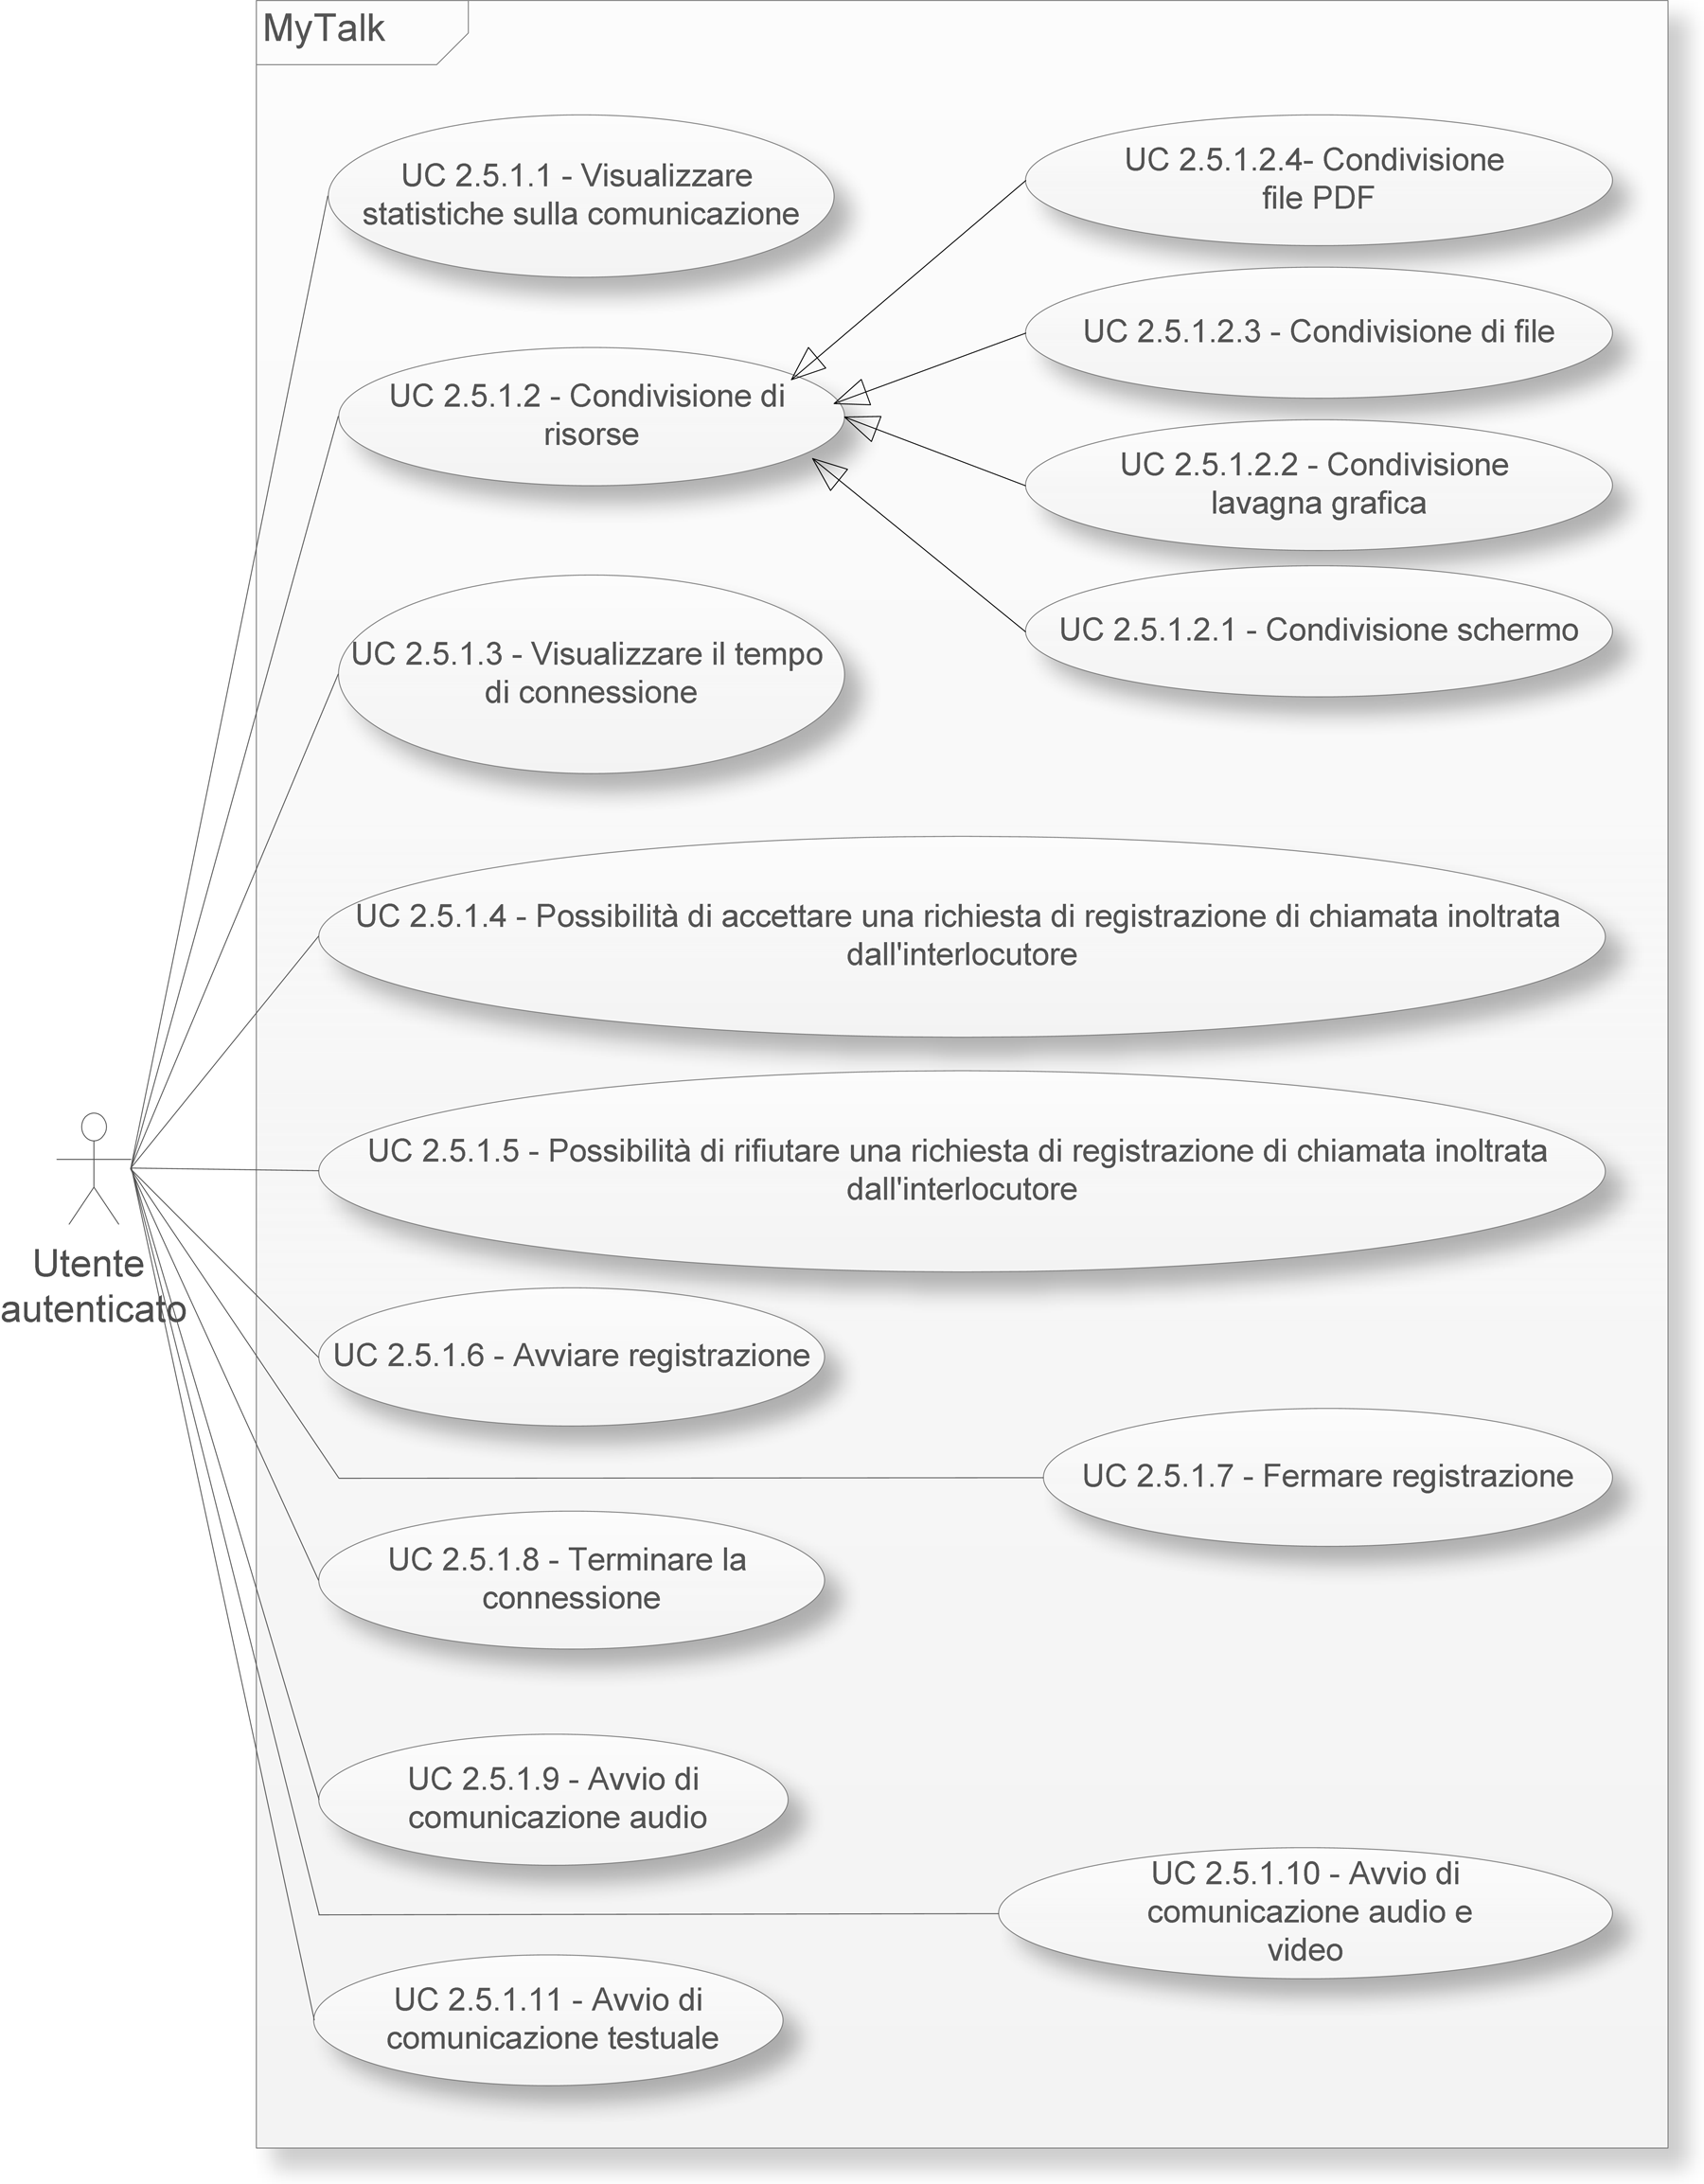
\includegraphics[width=.8\textwidth]{UC2-5-1}
\caption{}\label{fig:}
\end{center}
\end{figure}
\begin{description}
\item{\scshape\bfseries Attori principali:}Utente autenticato.
\item{\scshape\bfseries Scopo e descrizione:} Un utente, durante una chiamata audio, audio/video e chat, può eseguire diverse operazioni sulla connessione stabilita.
\item{\scshape\bfseries Precondizione:} L'utente è autenticato nel sistema, ed ha già stabilito una connessione con un utente autenticato.
\item{\scshape\bfseries Postcondizione:} L'utente ha concluso la comunicazione. La causa della terminazione può essere attribuita alla chiusura volontaria della connessione oppure al fatto che l'utente rimane l'unico attivo nella connessione.
\item{\scshape\bfseries Illustrazione scenario principale:} L'utente ha avviato una comunicazione. Mentre questa è in esecuzione, l'utente potrà: visualizzare le statistiche sulla comunicazione (UC2.5.1.1), condividere delle risorse dal proprio dispositivo (Condivisione di PDF, invio di file, condivisione di una lavagna grafica, e condivisione dello schermo)(UC2.5.1.2), visualizzare da quanto tempo è aperta la connessione (UC2.5.1.3), avviare e fermare una registrazione (UC2.5.1.6 - UC2.5.1.7), accettare o rifiutare una richiesta di registrazione inoltrata da un interlocutore (UC2.5.1.4 - UC2.5.1.5). Infine l'utente può decidere di terminare la comunicazione (UC2.5.1.8).
\end{description}

\subsection{UC2.5.1.1: Visualizzazione statistiche sulla comunicazione}
\begin{figure}[H]
\begin{center}
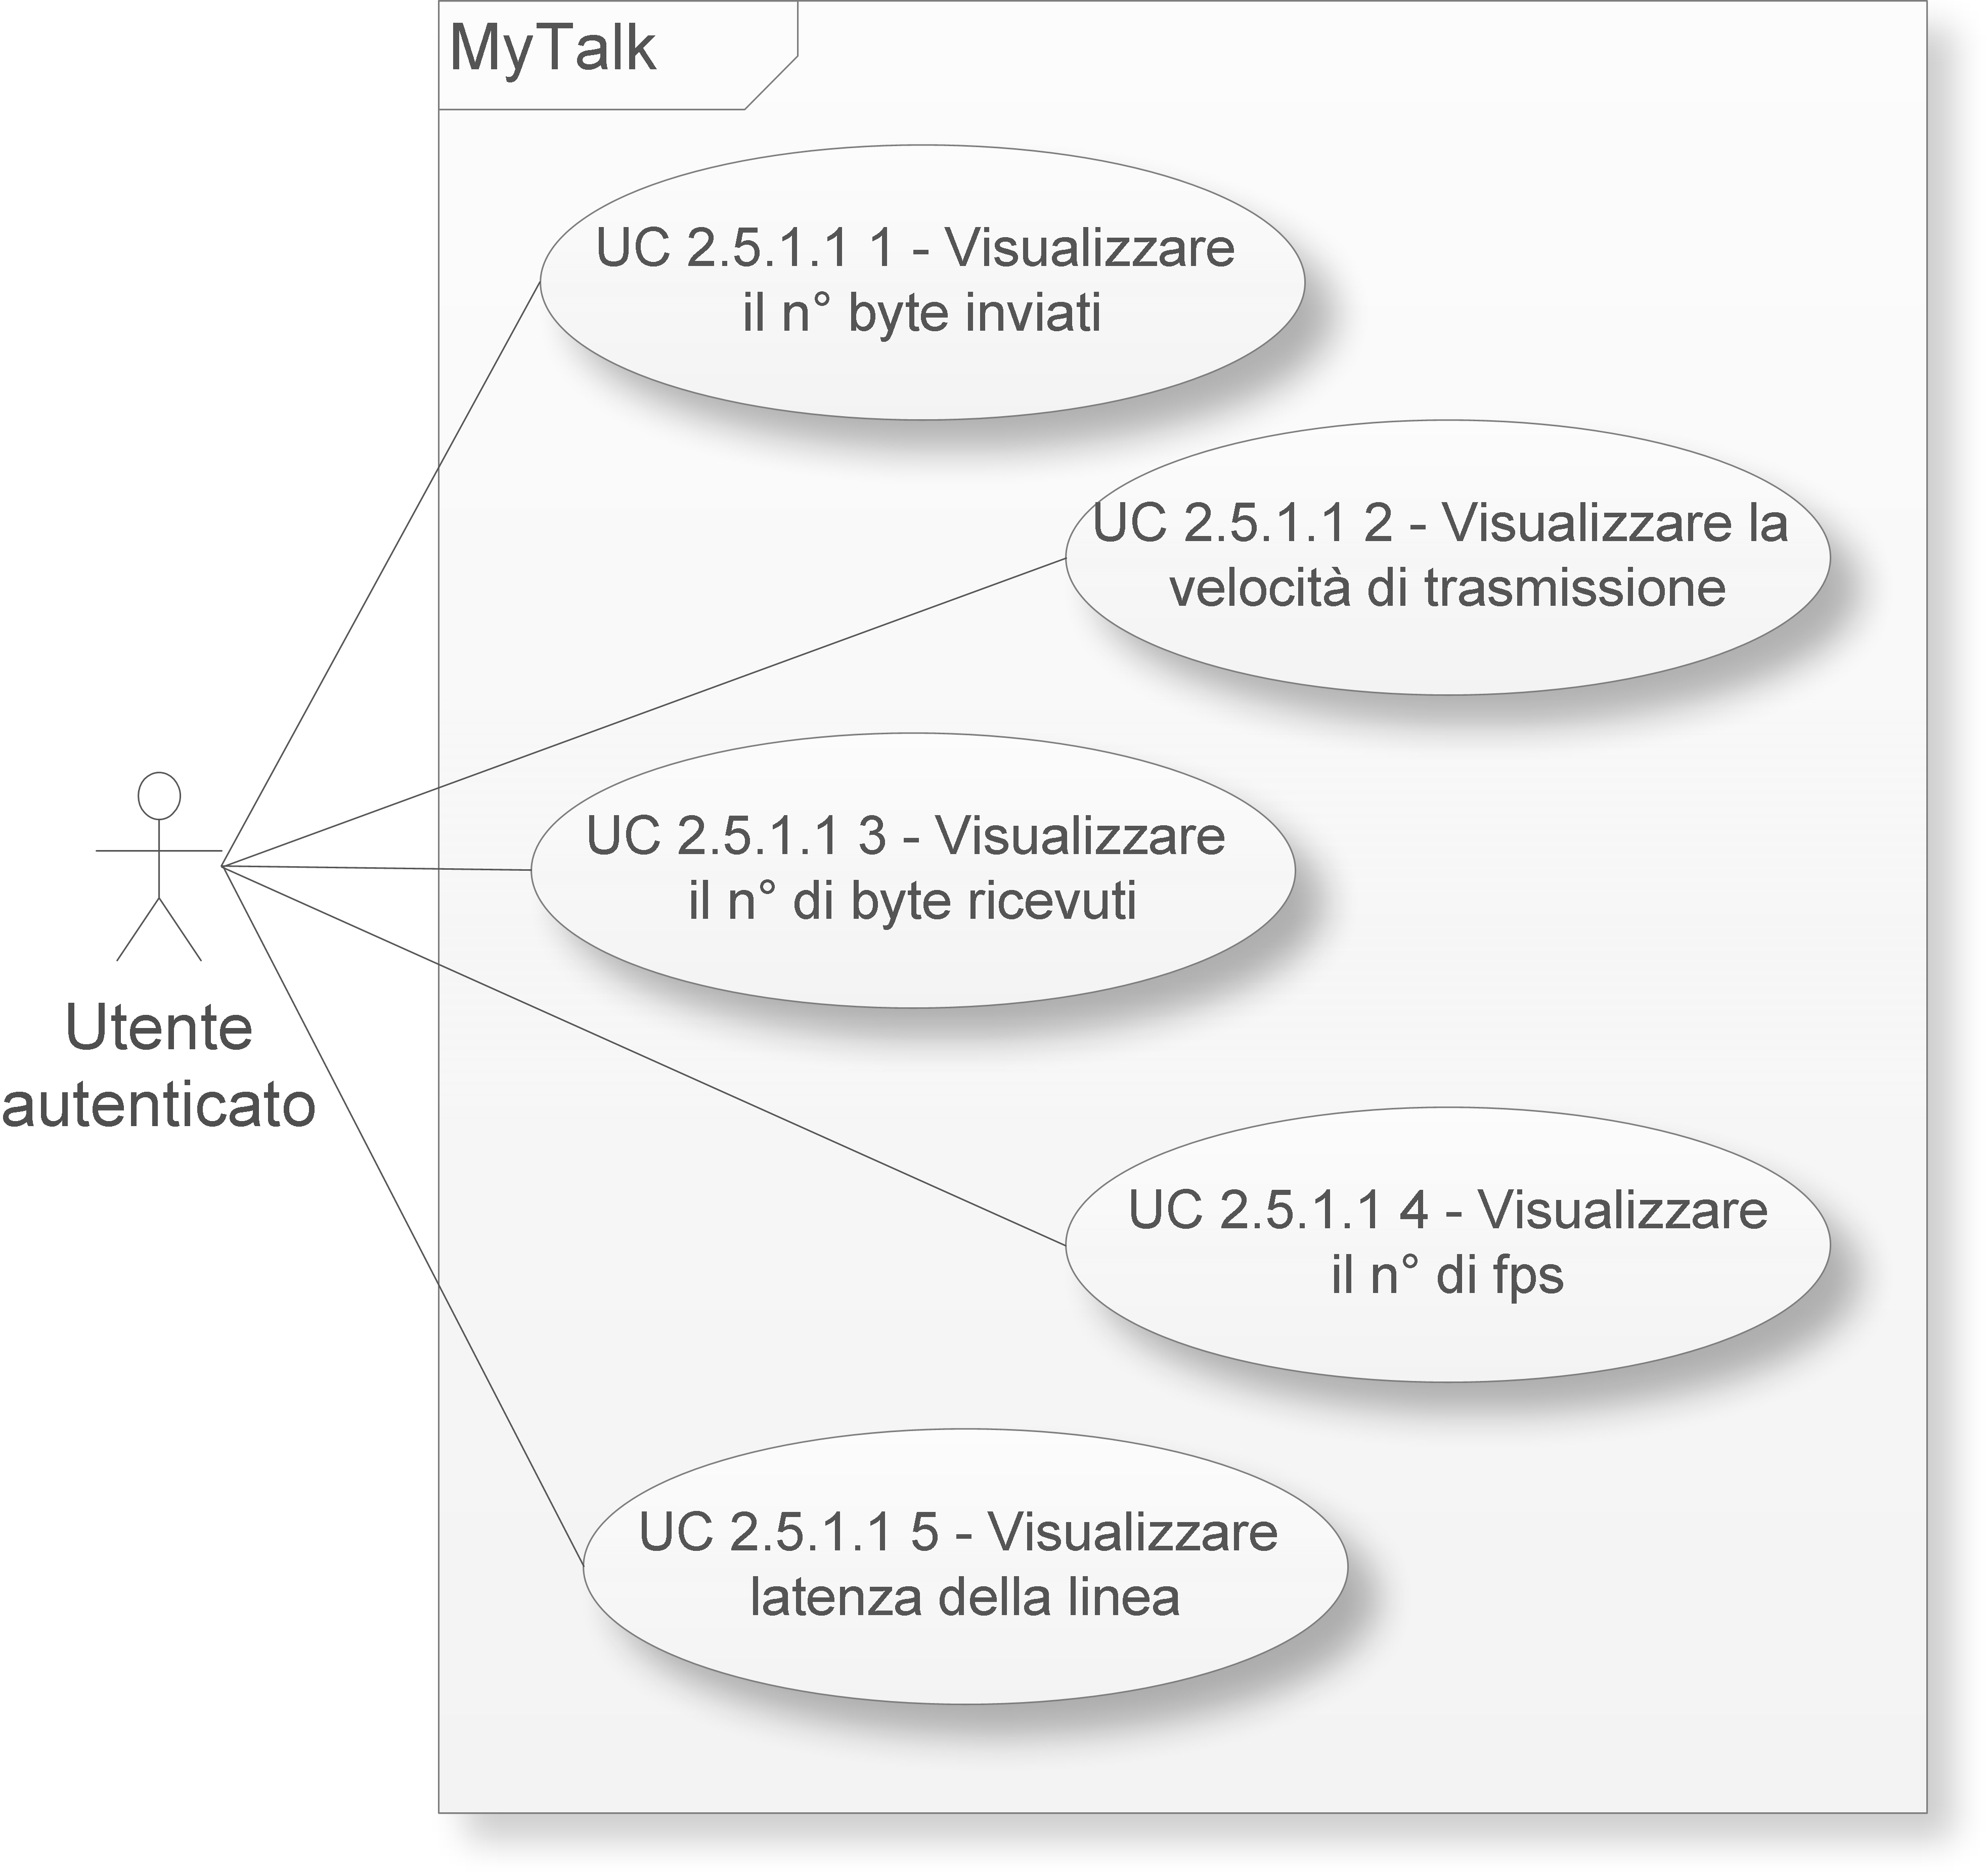
\includegraphics[width=.8\textwidth]{UC2-5-1-1}
\caption{}\label{fig:}
\end{center}
\end{figure}
\begin{description}
\item{\scshape\bfseries Attori principali:}Utente autenticato.
\item{\scshape\bfseries Scopo e descrizione:} L'utente visualizza i dettagli della comunicazione con un altro utente.
\item{\scshape\bfseries Precondizione:} L'utente sta comunicando con un altro utente del sistema.
\item{\scshape\bfseries Postcondizione:} L'utente ha visualizzato tutte le informazioni riguardanti la comunicazione.
\item{\scshape\bfseries Illustrazione scenario principale:} L'utente che comincia a comunicare con un altro utente ha a disposizione la visualizzazione di alcune informazioni sulla comunicazione in corso, come il numero di byte ricevuti ed inviati (UC2.5.1.1.1 - UC2.5.1.1.3), la latenza ossia il tempo che passa da quando un utente trasmette a quando l'altro utente riceve (UC2.5.1.1.5), la velocità di trasmissione dei dati (UC2.5.1.1.2) e i frame per secondo (fps) nel caso sia in corso una videochiamata (UC2.5.1.1.4).
\end{description}

\subsection{UC2.7: Ricerca di un utente}
\begin{figure}[H]
\begin{center}
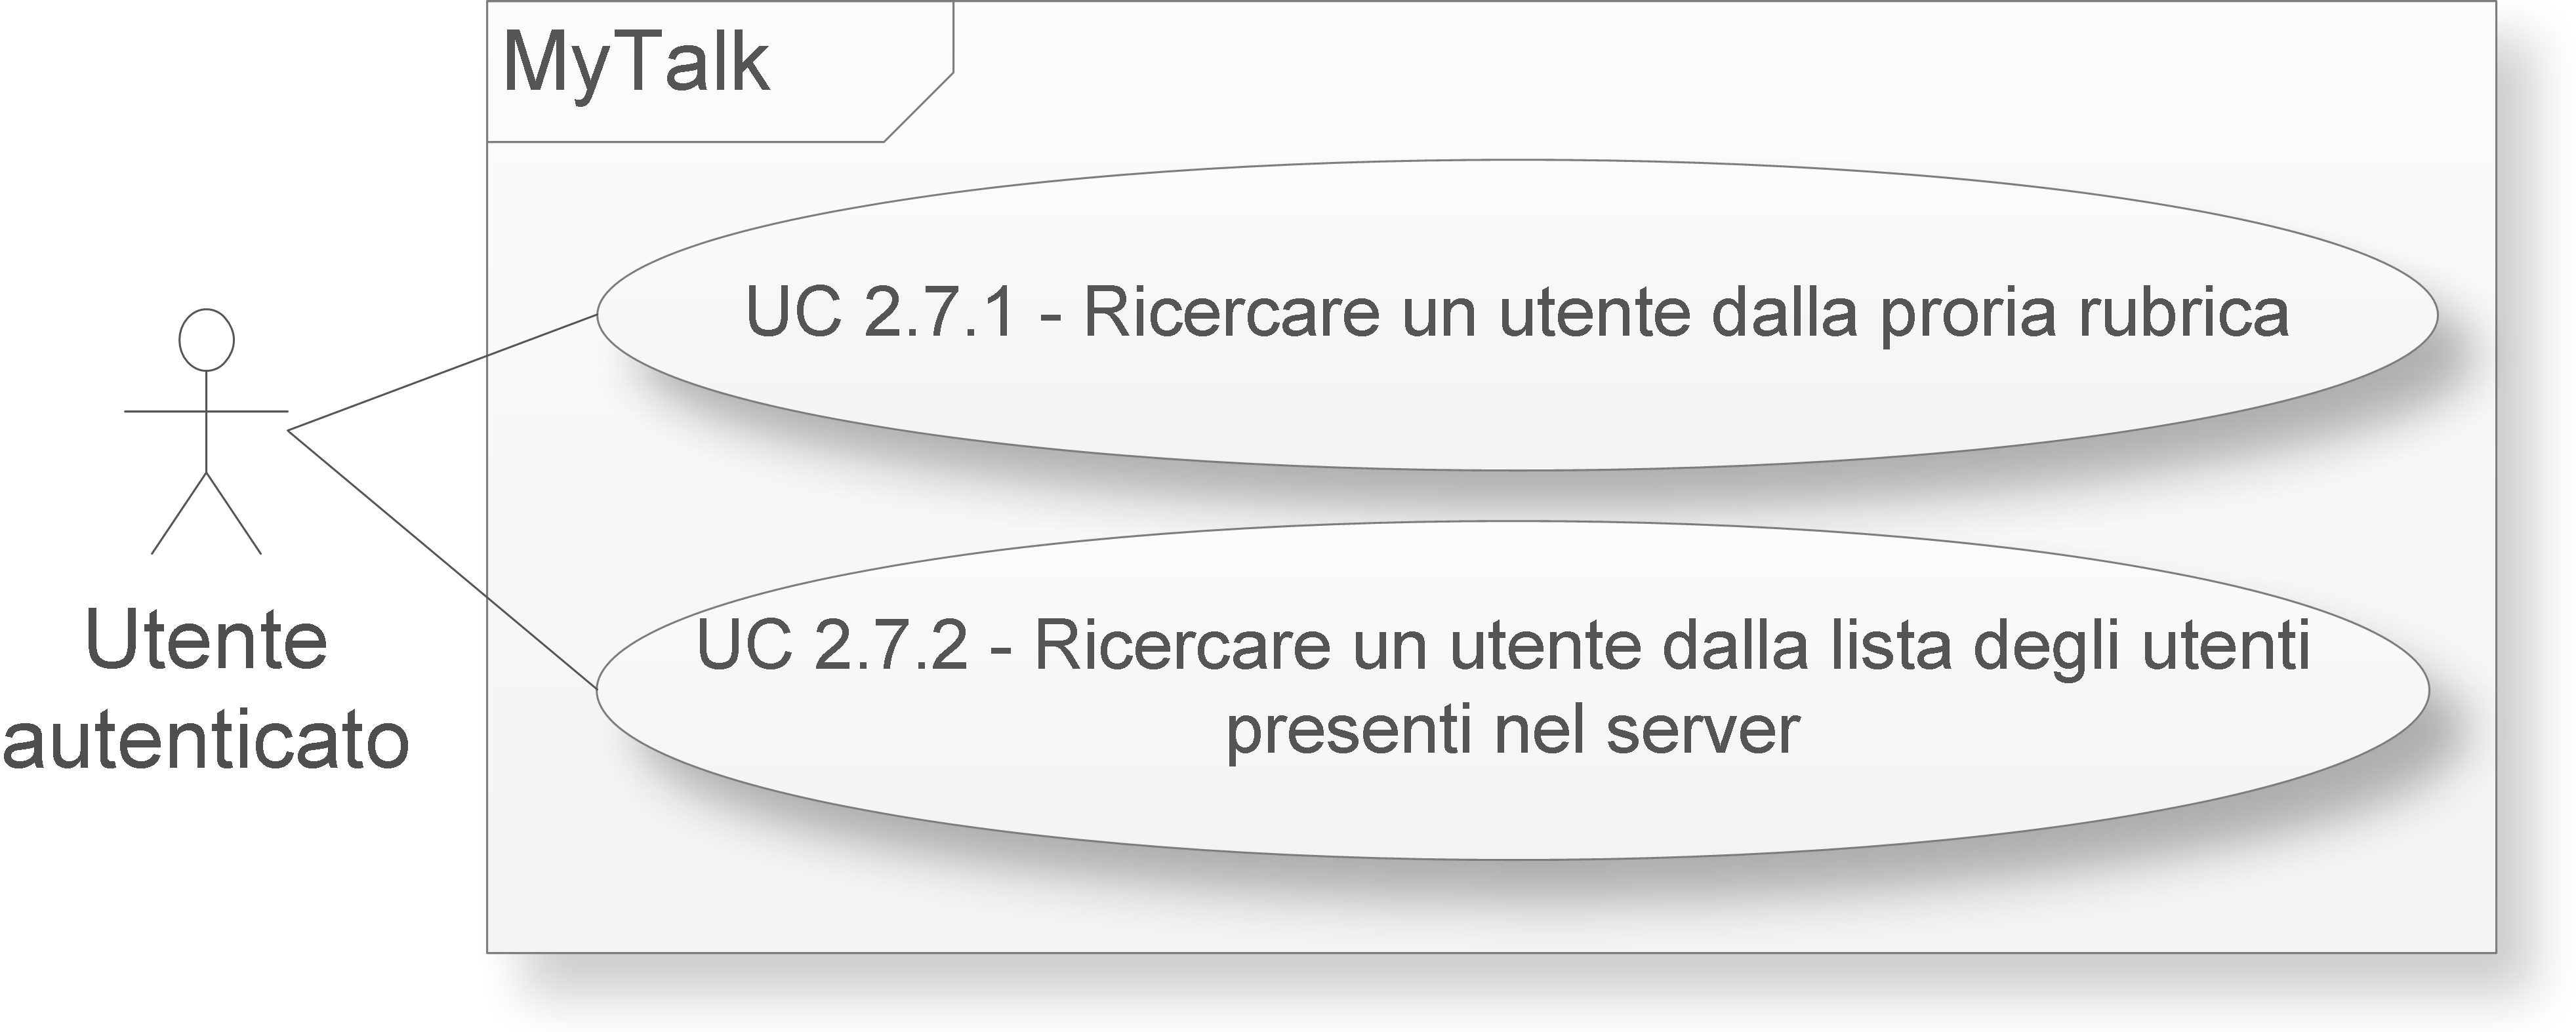
\includegraphics[width=.8\textwidth]{UC2-7}
\caption{}\label{fig:}
\end{center}
\end{figure}
\begin{description}
\item{\scshape\bfseries Attori principali:}Utente autenticato.
\item{\scshape\bfseries Scopo e descrizione:} L'utente desidera ricercare altri utenti all'interno del sistema.
\item{\scshape\bfseries Precondizione:} L'utente è autenticato al sistema; la lista degli utenti registrati presso il server non è vuota.
\item{\scshape\bfseries Postcondizione:} L'utente ha ottenuto una lista (possibilmente vuota) di utenti che soddisfano i parametri di ricerca.
\item{\scshape\bfseries Illustrazione scenario principale:} Nel momento in cui un utente vuole ricercare un altro utente registrato nel sistema, ha la possibilità  di ricercarlo o nella propria rubrica (UC2.7.1) o nella lista di utenti registrati nel sistema (UC2.7.2).
\end{description}

\newpage\section{Requisiti di prodotto}
I requisiti verranno suddivisi in base alla loro priorità. Rispettivamente seguirà la lista dei requisiti obbligatori, facoltativi e desiferabili. Ogni requisito è identificato con il seguente formato RXYZI con:


		\begin{itemize}

			\item \textbf{X}: indica la tipologia dell'utente interessato dal requisito. I possibili valori che X può assumere sono U (utente) oppure S (sistema).

			\item \textbf{Y}: indica la tipologia del requisito, e può assumere i valori: F(funzionale), Q(qualitativo), P(prestazionale), D(dichiarativo).

			\item \textbf{Z}: indica il livello di priorità del requisito. Può assumere i valori O(obbligatorio), \\F(facoltativo), D(desiderabile).

			\item \textbf{I}: indica l'id numerico del requisito, denominato secondo le direttive delle norme di progetto.

		\end{itemize}


		Ogni requisito si può suddividere in sottorequisiti. Tale evento è evidenziato dal valore del campo I, come riportato nelle norme di progetto. Infine i requisiti sono ordinati (nelle proprie sezioni) in base all'ordine crescente del campo numerico I.\
Per quanto riguarda invece i requisiti di processo, si rimanda ai documenti \textit{piano\_di\_qualifica.2.0.pdf} (sez. 3.1) e \textit{norme\_di\_progetto.2.0.pdf} (in particolare le sez. 2, 3 e 4).

\subsection{Requisiti funzionali}


\subsubsection{Requisiti funzionali obbligatori}

\begin{center}
\rowcolors{2}{lightblue}{llightblue}\begin{longtable}{lp{.55\textwidth}l}
\toprule Codice & Requisito & Fonte\\
\midrule
RUFO1.0.0 & L'utente deve potersi autentificare nel server, così da permettere a quest'ultimo di rilevare la sua presenza nel sistema. & Interno \\
RSFO1.2.0 & Per effettuare il login è necessario inserire i dati utente & Interno\\
RSFO1.2.1 & Per effettuare il login è necessario inserire il proprio username & Interno\\
RSFO1.2.2 & Per effettuare il login è necessario inserire la propria password & Interno\\
RUFO2.0.0 & Registrazione del nuovo utente & Capitolato d'appalto \\
RSFO2.1.0 & Inserimento dei dati obbligatori per l’autenticazione & Interno \\
RSFO2.1.3 & Inserimento del campo obbligatorio username (e-mail) & Interno\\
RSFO2.1.4 & Inserimento del campo obbligatorio password & Interno\\
RSFO2.1.5 & Inserimento del campo obbligatorio ``domanda segreta'' & Interno\\
RSFO2.1.6 & Inserimento del campo obbligatorio ``risposta alla domanda segreta'' & Interno\\
RUFO5.0.0 & Possibilità di visualizzare la lista di utenti registrati nel sistema & Capitolato d'appalto \\
RUFO6.1.0 & stabilire una comunicazione audio con un utente in linea & Capitolato d'appalto \\
RUFO6.1.1 & Stabilire una comunicazione audio mediante inserimento d'indirizzo IP & Capitolato d'appalto \\
RUFO6.1.3 & Stabilire una comunicazione audio con un utente registrato e NON presente nella rubrica & Capitolato d'appalto \\
RUFO6.2.0 & Stabilire una comunicazione audio e video con un utente in linea & Capitolato d'appalto \\
RUFO6.2.1 & Stabilire una comunicazione audio e video mediante inserimento d'indirizzo IP & Capitolato d'appalto \\
RUFO6.2.3 & Stabilire una comunicazione audio e video con un utente registrato e NON presente nella rubrica & Capitolato d'appalto \\
RUFO6.4.0 & Mantenere la comunicazione audio e video fino a che uno dei due utenti non la chiude & Capitolato d'appalto \\
RUFO6.5.0 & Mantenere la comunicazione audio fino a che uno dei due utenti non la chiude & Capitolato d'appalto \\
RUFO7.0.0 & Indicare il tempo di comunicazione & Capitolato d'appalto \\
RUFO8.0.0 & Valutare il numero di byte trasmessi & Capitolato d'appalto \\
RUFO8.1.0 & Valutare il numero di byte inviati & Interno \\
RUFO8.2.0 & Valutare il numero di byte ricevuti & Interno \\
RUFO9.0.0 & Indicare la qualità della linea di trasmissione & Capitolato d'appalto \\
RUFO9.1.0 & Rilevare latenza & Capitolato d'appalto \\
RUFO9.2.0 & Rilevare velocità di trasmissione & Capitolato d'appalto \\
RSFO11.0.0 & Creare una connessione tra client, mediante l'utilizzo di un server & Capitolato d'appalto \\
RSFO11.1.0 & Utilizzo del protocollo webSocket per creare una connessione tra 2 utenti & Interno \\
RSFO12.0.0 & Gestire gli eventi dell'utente durante la connessione. & Interno \\
RUFO12.3.0 & Chi partecipa alla connessione può togliersi da essa & Interno \\
\bottomrule
\end{longtable}
\end{center}

\subsubsection{Requisiti funzionali desiderabili}

\begin{center}
\rowcolors{2}{lightblue}{llightblue}\begin{longtable}{lp{.55\textwidth}l}
\toprule Codice & Requisito & Fonte\\
\midrule
RUFD1.1.0 & Gestione password dimenticata & Interno \\
RUFD1.1.1 & Proporre la domanda segreta all'utente & Interno \\
RUFD1.1.2 & Invio di una mail all'utente contenete la password dimenticata & Interno \\
RSFD2.1.2 & Convalidare username (e-mail) dell'utente & Interno \\
RUFD12.2.0 & Chi crea la connessione può eliminare i membri del gruppo di chiamata & Interno \\
RUFD13.1.0 & Servizio chat tra 2 utenti & Interno \\
RSFD21.0.0 & Gestione interfaccia grafica in più lingue & Interno \\
\bottomrule
\end{longtable}
\end{center}

\subsubsection{Requisiti funzionali facoltativi}

\begin{center}
\rowcolors{2}{lightblue}{llightblue}\begin{longtable}{lp{.55\textwidth}l}
\toprule Codice & Requisito & Fonte\\
\midrule
RUFF3.0.0 & Modifica dati utente & Interno \\
RUFF3.1.0 & Modifica dei dati per l'autenticazione & Interno \\
RUFF3.1.1 & Modifica della password & Interno\\
RUFF3.1.2 & Modifica della ``domanda segreta'' & Interno\\
RUFF3.1.3 & Modifica della ``risposta alla domanda segreta'' & Interno\\
RUFF3.2.0 & Modifica dei dati anagrafici facoltativi & Interno \\
RUFF3.2.1 & Modifica del nome & Interno\\
RUFF3.2.2 & Modifica del cognome & Interno\\
RUFF3.2.3 & Modifica dell'immagine profilo & Interno\\
RUFF4.0.0 & L'utente ha a disposizione una rubrica personale & Interno \\
RUFF4.1.0 & Possibilità d'inserire utenti nella propria rubrica & Capitolato d'appalto \\
RUFF4.2.0 & Possibilità di eliminare un utente dalla propria rubrica & Interno \\
RUFF4.3.0 & Possibilità di ordinare la rubrica su alcuni parametri rilevanti & Interno \\
RUFF4.3.1 & Possibilità di ordinare la rubrica in relazione al nome utente & Interno\\
RUFF4.3.2 & Possibilità di ordinare la rubrica in relazione al nome dei gruppi & Interno\\
RUFF4.4.0 & Possibilità di suddividere la rubrica in gruppi & Interno \\
RUFF4.4.1 & Possibilità di togliere un elemento da un gruppo & Interno \\
RUFF4.4.2 & Possibilità di aggiungere un elemento in un gruppo & Interno \\
RUFF4.4.3 & Possibilità di creare un gruppo & Interno \\
RUFF4.4.4 & Possibilità di eliminare un gruppo & Interno \\
RUFF4.5.0 & Possibilità di esportare in xml la rubrica personale & Interno \\
RUFF4.6.0 & Possibilità di modificare la rubrica importando un file xml & Interno \\
RUFF4.7.0 & Ricerca di un utente nella propria rubrica. & Interno \\
RUFF4.7.1 & Ricerca degli utenti nel cui nome compare la parola ricercata & Interno\\
RUFF4.7.2 & Ricerca degli utenti nel cui cognome compare la parola ricercata & Interno\\
RUFF4.7.3 & Ricerca degli utenti appartenenti ad un gruppo nel cui nome compare la parola ricercata & Interno\\
RUFF5.1.0 & Possibilità di cercare un utente dalla lista & Interno \\
RUFF5.1.1 & Possibilità di cercare un utente dalla lista, in relazione al nome utente & Interno\\
RUFF5.1.2 & Possibilità di cercare un utente dalla lista, in relazione al email & Interno\\
RUFF6.1.2 & Stabilire una comunicazione audio con un utente registrato e presente nella rubrica & Capitolato d'appalto \\
RUFF6.1.4 & Promuovere una comunicazione audio avviata con un utente in una comunicazione audio e video & Interno \\
RUFF6.2.2 & Stabilire una comunicazione audio e video con un utente presente nella rubrica & Capitolato d'appalto \\
RUFF6.2.4 & Declassare una comunicazione audio e video avviata con un utente in una comunicazione solo audio & Interno \\
RUFF6.2.5 & Disattivare la webcam utente pur continuando a ricevere il segnale video proveniente dall'altro capo della comunicazione & Interno \\
RUFF6.3.0 & Disattivare il microfono utente pur continuando a ricevere il segnale video proveniente dall'altro capo della comunicazione & Interno \\
RUFF9.3.0 & Rilevazione frame per secondo & Interno \\
RSFF11.2.0 & Utilizzo del protocollo webSocket per creare una connessione tra più di 2 utenti & Interno \\
RSFF12.1.0 & Estendere la connessione ad altri client & Interno \\
RUFF13.0.0 & Servizio chat testuale & Capitolato d'appalto \\
RUFF13.2.0 & Servizio chat tra più di 2 utenti & Interno \\
RUFF14.0.0 & Registrazione della chiamata & Capitolato d'appalto \\
RUFF14.1.0 & Necessità di autorizzazione dagli utenti della chiamata per poter avviare la registrazione & Interno \\
RUFF14.2.0 & Registrazione audio & Interno \\
RUFF14.3.0 & Possibilità di riascoltare la registrazione & Interno \\
RUFF15.0.0 & L'utente avrà a disposizione una segreteria telefonica. & Interno \\
RUFF15.1.0 & Possibilità di lasciare un audio messaggio in segreteria & Interno \\
RUFF15.2.0 & Possibilità di lasciare un audio e video messaggio in segreteria & Capitolato d'appalto \\
RUFF15.3.0 & Possibilità di ascoltare la propria segreteria & Interno \\
RUFF15.4.0 & Possibilità di cancellare messaggi della segretaria & Interno \\
RUFF15.5.0 & Possibilità di cambiare lo stato del messaggio da "non ascoltato" a "ascoltato" & Interno \\
RUFF16.0.0 & Fornire la possibilità di cambiare lo stato utente & Interno \\
RUFF16.1.0  & Fornire la possibilità di impostare 'disponibile' come stato utente & Interno \\
RUFF16.2.0 & Fornire la possibilità di impostare 'non disponibile' come stato utente & Interno \\
RUFF17.0.0 & Dare la possibilità di vedere gli stati personali altrui. & Interno \\
RUFF18.0.0 & Presenza di una Blacklist & Interno \\
RUFF19.0.0 & Presenza di uno storico delle chiamate & Interno \\
RUFF20.0.0 & Condividere risorse & Interno \\
RUFF20.1.0 & Condivisione del monitor & Interno \\
RUFF20.2.0 & Condivisione pdf & Interno \\
RUFF20.3.0 & Condivisione lavagna grafica. & Interno \\
RUFF20.4.0 & Invio file & Interno \\
\bottomrule
\end{longtable}
\end{center}

\subsection{Requisiti qualitativi}

\subsubsection{Requisiti qualitativi obbligatori}

\begin{center}
\rowcolors{2}{lightblue}{llightblue}\begin{longtable}{lp{.55\textwidth}l}
\toprule Codice & Requisito & Fonte\\
\midrule
RSQO6.4.0 & L'applicativo dev'essere predisposto a facili modifiche dettate da evoluzioni future di WebRTC. & Capitolato d'appalto \\
\bottomrule
\end{longtable}
\end{center}

\begin{center}
\rowcolors{2}{lightblue}{llightblue}\begin{longtable}{lp{.55\textwidth}l}
\toprule Codice & Requisito & Fonte\\
\midrule
RSQF23.0.0 & Verificare che l'applicativo funzioni anche sotto gli altri browser del S.O. Windows & Interno \\
RSQF23.1.0 & Verificare che funzioni con Opera (versione 12.0 minima) & Capitolato d'appalto \\
RSQF23.2.0 & Verificare che funzioni con Firefox (versione 17.0 minima) & Capitolato d'appalto \\
RSQF23.3.0 & Verificare che funzioni con Internet Explorer (versione 10.0 minima) & Capitolato d'appalto \\
RSQF23.4.0 & Verificare che funzioni con Safari (versione 6.0 minima) & Capitolato d'appalto \\
RSQF24.0.0 & Verificare che l'applicativo funzioni anche sotto gli altri browser del S.O. Linux & Interno \\
RSQF24.1.0 & Verificare che funzioni con Opera (versione 12.0 minima) & Capitolato d'appalto \\
RSQF24.2.0 & Verificare che funzioni con Firefox (versione 17.0 minima) & Capitolato d'appalto \\
RSQF24.3.0 & Verificare che funzioni con Chromium (versione 25.0.1313 minima) & Interno \\
RSQF25.0.0 & Verificare che l'applicativo funzioni anche sotto gli altri browser del S.O. Macintosh & Interno \\
RSQF25.1.0 & Verificare che funzioni con Opera (versione 12.0 minima) & Capitolato d'appalto \\
RSQF25.2.0 & Verificare che funzioni con Firefox (versione 17.0 minima) & Capitolato d'appalto \\
RSQF25.3.0 & Verificare che funzioni con Safari  (versione 6.0 minima) & Capitolato d'appalto \\
RSQF26.0.0 & Il software dovrà essere compatibile con componenti realizzati in Flash & Capitolato d'appalto \\
\bottomrule
\end{longtable}
\end{center}

\subsection{Requisiti dichiarativi}

\subsubsection{Requisiti dichiarativi obbligatori}

\begin{center}
\rowcolors{2}{lightblue}{llightblue}\begin{longtable}{lp{.55\textwidth}l}
\toprule Codice & Requisito & Fonte\\
\midrule
RSDO6.0.0 & Gestire le comunicazioni utente tramite WebRTC & Capitolato d'appalto \\
RSDO10.0.0 & L'intero sistema deve essere contenuto in un unica pagina Web & Capitolato d'appalto \\
RSDO10.1.0 & L'interfaccia grafica non deve subire refresh per ogni operazione dell'utente & Interno \\
RSDO11.3.0 & Il server sarà implementato tramite il linguaggio Java. & Capitolato d'appalto \\
RSDO11.4.0 & Il server sarà coinvolto solo per avviare la comunicazione & Capitolato d'appalto \\
RSDO22.0.0 & L'applicativo deve essere fruibile attraverso un browser web & Capitolato d'appalto \\
RSDO22.1.0 & L'applicativo web deve funzionare nel browser web Google Chrome (versione minima 23.0.1271.97m) & Capitolato d'appalto \\
\bottomrule
\end{longtable}
\end{center}

\subsubsection{Requisiti dichiarativi desiderabili}

\begin{center}
\rowcolors{2}{lightblue}{llightblue}\begin{longtable}{lp{.55\textwidth}l}
\toprule Codice & Requisito & Fonte\\
\midrule
RSDD2.1.1 & L'utente ha una stima per la complessità della propria password & Interno \\
RSDD2.2.0 & Inserimento dei dati facoltativi riferiti all'anagrafica & Interno \\
\bottomrule
\end{longtable}
\end{center}

\begin{center}
\rowcolors{2}{lightblue}{llightblue}\begin{longtable}{lp{.55\textwidth}l}
\toprule Codice & Requisito & Fonte\\
\midrule
\bottomrule
\end{longtable}
\end{center}

\newpage
\section{Requisiti di qualità di processo}\label{sec:qualitaProcesso}

Al fine di introdurre qualità nei processi implementati per la creazione del prodotto, il team ha ritenuto necessario identificare dei requisiti da tenere in considerazione nelle scelta delle attività e nella loro pianificazione. Per la loro peculiarità e la sostanziale separazione dai requisiti di prodotto, i requisiti di processo sono stati riportati in una sezione separata da quest'ultimi. Di seguito è riportata la tabella dei requisiti evidenziati.

Il sistema di nominazione è analogo a quello usato nei ``Requisiti di prodotto'' e nello specifico tali requisiti saranno identificati come RSQO (requisiti obbligatori di qualità di sistema).

\begin{center}
\rowcolors{2}{lightblue}{llightblue}\begin{longtable}{lp{.55\textwidth}l}
\toprule Codice & Requisito & Fonte\\
\midrule
RSQO27.0.0 & il modello SPY e CMMI sono utilizzati per valutare la qualità dei processi & Interno \\
RSQO28.0.0 & Gli standard di qualità hanno come riferimento lo standard ISO/9126:2001 & Interno \\
RSQO28.1.0 & Adozione del ciclo di Deming (PDCA) per valutare e migliorare i processi & Interno \\
RSQO29.0.0 & Distinte modalità di verifica per ogni attività durante il ciclo di vita progettuale & Interno \\
RSQO29.1.0 & Modalità di verifica specifiche per l'analisi dei requisiti & Interno \\
RSQO29.2.0 & Modalità di verifica specifiche per la progettazione di alto livello & Interno \\
RSQO29.3.0 & Modalità di verifica specifiche per la progettazione di dettaglio & Interno \\
RSQO29.4.0 & Modalità di verifica specifiche per la codifica & Interno \\
RSQO29.4.1 & Utilizzo di metriche specifiche per valutare il codice & Interno \\
RSQO29.5.0 & Modalità di verifica specifiche per validazione & Interno \\
RSQO30.0.0 & Uso di un sistema di ticketing (tracciato) per evidenziare e risolvere errori o problematiche & Interno \\
RSQO31.0.0 & l'attività di progettazione condotta nel rispetto dei principi della programmazione ad oggetti & Interno \\
RSQO31.1.0 & durante la progettazione è imposto l'utilizzo di interfacce & Interno \\
RSQO31.2.0 & il processo di individuazione delle classi e il loro corrispettivo inserimento in una componente è giustificato dal significato e dall'utilizzo della classe stessa (principio di coesione) & Interno \\
\bottomrule
\end{longtable}
\end{center}

\newpage\section{Tracciamento use case - requisiti}\label{sec:tracciamento}

\begin{center}
\rowcolors{2}{lightblue}{llightblue}\begin{longtable}{lp{.55\textwidth}l}
\toprule Codice UC & Nome UC  & Requisito\\
\midrule
UC1 & Login e registrazione & RUFO1.0.0 \\
 &  & RUFD1.1.0 \\
 &  & RUFD1.1.1 \\
 &  & RUFD1.1.2 \\
 &  & RSFO1.2.0 \\
 &  & RSFO1.2.1 \\
 &  & RSFO1.2.2 \\
 &  & RUFO2.0.0 \\
 &  & RSFO2.1.0 \\
 &  & RSDD2.1.1 \\
 &  & RSFO2.1.3 \\
 &  & RSFO2.1.4 \\
 &  & RSFO2.1.5 \\
 &  & RSFO2.1.6 \\
 &  & RSFD2.1.2 \\
 &  & RSDD2.2.0 \\
UC2 & Home screen dell'applicativo & RUFF3.0.0 \\
 &  & RUFF3.1.0 \\
 &  & RUFF3.1.1 \\
 &  & RUFF3.1.2 \\
 &  & RUFF3.1.3 \\
 &  & RUFF3.2.1 \\
 &  & RUFF3.2.2 \\
 &  & RUFF3.2.3 \\
 &  & RUFF3.2.0 \\
 &  & RUFF4.0.0 \\
 &  & RUFF4.1.0 \\
 &  & RUFF4.2.0 \\
 &  & RUFF4.3.0 \\
 &  & RUFF4.3.1 \\
 &  & RUFF4.3.2 \\
 &  & RUFF4.4.0 \\
 &  & RUFF4.4.1 \\
 &  & RUFF4.4.2 \\
 &  & RUFF4.4.3 \\
 &  & RUFF4.4.4 \\
 &  & RUFF4.5.0 \\
 &  & RUFF4.6.0 \\
 &  & RUFF4.7.0 \\
 &  & RUFF4.7.1 \\
 &  & RUFF4.7.2 \\
 &  & RUFF4.7.3 \\
 &  & RUFO5.0.0 \\
 &  & RUFF5.1.0 \\
 &  & RUFF5.1.1 \\
 &  & RUFF5.1.2 \\
 &  & RUFO6.1.0 \\
 &  & RUFO6.1.1 \\
 &  & RUFF6.1.2 \\
 &  & RUFO6.1.3 \\
 &  & RUFF6.1.4 \\
 &  & RUFO6.2.0 \\
 &  & RUFO6.2.1 \\
 &  & RUFF6.2.2 \\
 &  & RUFO6.2.3 \\
 &  & RUFF6.2.4 \\
 &  & RUFF6.2.5 \\
 &  & RUFF6.3.0 \\
 &  & RUFO7.0.0 \\
 &  & RUFO8.0.0 \\
 &  & RUFO8.1.0 \\
 &  & RUFO8.2.0 \\
 &  & RUFO9.0.0 \\
 &  & RUFO9.1.0 \\
 &  & RUFO9.2.0 \\
 &  & RUFF9.3.0 \\
 &  & RSFF12.1.0 \\
 &  & RUFD12.2.0 \\
 &  & RUFO12.3.0 \\
 &  & RUFF13.0.0 \\
 &  & RUFD13.1.0 \\
 &  & RUFF13.2.0 \\
 &  & RUFF14.0.0 \\
 &  & RUFF14.1.0 \\
 &  & RUFF14.2.0 \\
 &  & RUFF15.0.0 \\
 &  & RUFF15.1.0 \\
 &  & RUFF15.2.0 \\
 &  & RUFF15.3.0 \\
 &  & RUFF15.4.0 \\
 &  & RUFF15.5.0 \\
 &  & RUFF16.0.0 \\
 &  & RUFF17.0.0 \\
 &  & RUFF18.0.0 \\
 &  & RUFF19.0.0 \\
 &  & RUFF20.0.0 \\
 &  & RUFF20.1.0 \\
 &  & RUFF20.2.0 \\
 &  & RUFF20.3.0 \\
 &  & RUFF20.4.0 \\
UC1.1 & Login utente & RUFO1.0.0 \\
 &  & RSFO1.2.0 \\
UC1.2 & Registrazione & RUFO2.0.0 \\
 &  & RSFO2.1.0 \\
 &  & RSDD2.1.1 \\
 &  & RSFD2.1.2 \\
 &  & RSFO2.1.3 \\
 &  & RSFO2.1.4 \\
 &  & RSFO2.1.5 \\
 &  & RSFO2.1.6 \\    
 &  & RSDD2.2.0 \\
UC1.3 & Recupero della password & RUFD1.1.0 \\
 &  & RUFD1.1.1 \\
 &  & RUFD1.1.2 \\
UC2.1 & Gestione account & RUFF3.0.0 \\
 &  & RUFF3.1.0 \\
 &  & RUFF3.1.1 \\
 &  & RUFF3.1.2 \\
 &  & RUFF3.1.3 \\
 &  & RUFF3.2.0 \\
UC2.2 & Gestire lo stato & RUFF16.0.0 \\
UC2.3 & Gestione della rubrica & RUFF4.0.0 \\
 &  & RUFF4.1.0 \\
 &  & RUFF4.2.0 \\
 &  & RUFF4.3.0 \\
 &  & RUFF4.3.1 \\
 &  & RUFF4.3.2 \\
 &  & RUFF4.4.0 \\
 &  & RUFF4.4.1 \\
 &  & RUFF4.4.2 \\
 &  & RUFF4.4.3 \\
 &  & RUFF4.4.4 \\
 &  & RUFF4.5.0 \\
 &  & RUFF4.6.0 \\
 &  & RUFF4.7.0 \\
 &  & RUFF4.7.1 \\
 &  & RUFF4.7.2 \\
 &  & RUFF4.7.3 \\
 &  & RUFO5.0.0 \\
 &  & RUFF5.1.0 \\
 &  & RUFF5.1.1 \\
 &  & RUFF5.1.2 \\
 &  & RUFF18.0.0 \\
UC2.4 & Gestire segreteria personale & RUFF15.0.0 \\
 &  & RUFF15.1.0 \\
 &  & RUFF15.2.0 \\
 &  & RUFF15.3.0 \\
 &  & RUFF15.4.0 \\
 &  & RUFF15.5.0 \\
UC2.7 & Ricerca di un utente & RUFF4.7.0 \\
 &  & RUFF4.7.1 \\
 &  & RUFF4.7.2 \\
 &  & RUFF4.7.3 \\
 &  & RUFF5.1.0 \\
 &  & RUFF5.1.1 \\
 &  & RUFF5.1.2 \\
UC2.5.1 & Connessione con altri utenti autenticati & RUFO6.1.0 \\
 &  & RUFO6.1.1 \\
 &  & RUFF6.1.2 \\
 &  & RUFO6.1.3 \\
 &  & RUFF6.1.4 \\
 &  & RUFO6.2.0 \\
 &  & RUFO6.2.1 \\
 &  & RUFF6.2.2 \\
 &  & RUFO6.2.3 \\
 &  & RUFF6.2.4 \\
 &  & RUFF6.2.5 \\
 &  & RUFF6.3.0 \\
 &  & RUFO7.0.0 \\
 &  & RUFO8.0.0 \\
 &  & RUFO8.1.0 \\
 &  & RUFO8.2.0 \\
 &  & RUFO9.0.0 \\
 &  & RUFO9.1.0 \\
 &  & RUFO9.2.0 \\
 &  & RUFF9.3.0 \\
 &  & RSFO12.0.0 \\
 &  & RSFF12.1.0 \\
 &  & RUFD12.2.0 \\
 &  & RUFO12.3.0 \\
 &  & RUFF13.0.0 \\
 &  & RUFD13.1.0 \\
 &  & RUFF13.2.0 \\
 &  & RUFF14.0.0 \\
 &  & RUFF14.1.0 \\
 &  & RUFF14.2.0 \\
 &  & RUFF20.0.0 \\
 &  & RUFF20.1.0 \\
 &  & RUFF20.2.0 \\
 &  & RUFF20.3.0 \\
 &  & RUFF20.4.0 \\
UC2.5.1.1 & Visualizzazione statistiche sulla comunicazione & RUFO7.0.0 \\
 &  & RUFO8.0.0 \\
 &  & RUFO8.1.0 \\
 &  & RUFO8.2.0 \\
 &  & RUFO9.0.0 \\
 &  & RUFO9.1.0 \\
 &  & RUFO9.2.0 \\
 &  & RUFF9.3.0 \\
\bottomrule
\end{longtable}
\end{center}
\newpage\section{Tracciamento requisiti - use case}\label{sec:tracciamento}

\begin{center}
\rowcolors{2}{lightblue}{llightblue}\begin{longtable}{lp{.55\textwidth}l}
\toprule Requisito & Codice UC\\
\midrule
RUFO1.0.0 & UC1 \\
 & UC1.1 \\
RUFD1.1.0 & UC1 \\
 & UC1.3 \\
RUFD1.1.1 & UC1 \\
 & UC1.3 \\
RUFD1.1.2 & UC1 \\
 & UC1.3 \\
RSFO1.2.0 & UC1 \\
 & UC1.1 \\
RSFO1.2.1 & UC1 \\
 & UC1.1 \\
RSFO1.2.2 & UC1 \\
 & UC1.1 \\ 
RUFO2.0.0 & UC1 \\
 & UC1.2 \\
RSFO2.1.0 & UC1 \\
 & UC1.2 \\
RSDD2.1.1 & UC1 \\
 & UC1.2 \\
RSFD2.1.2 & UC1 \\
 & UC1.2 \\
RSFO2.1.3 & UC1\\
 & UC2\\
RSFO2.1.4 & UC1\\
 & UC2\\
RSFO2.1.5 & UC1\\
 & UC2\\
RSFO2.1.6 & UC1\\
 & UC2\\
RSDD2.2.0 & UC1 \\
 & UC1.2 \\
RUFF3.0.0 & UC2 \\
 & UC2.1 \\
RUFF3.1.0 & UC2 \\
 & UC2.1 \\
RUFF3.1.1 & UC2 \\
 & UC2.1 \\
RUFF3.1.2 & UC2 \\
 & UC2.1 \\
RUFF3.1.3 & UC2 \\
 & UC2.1 \\
RUFF3.2.0 & UC2 \\
 & UC2.1 \\
RUFF3.2.1 & UC2 \\
 & UC2.1 \\
RUFF3.2.2 & UC2 \\
 & UC2.1 \\
RUFF3.2.3 & UC2 \\
 & UC2.1 \\
RUFF4.0.0 & UC2 \\
 & UC2.3 \\
RUFF4.1.0 & UC2 \\
 & UC2.3 \\
RUFF4.2.0 & UC2 \\
 & UC2.3 \\
RUFF4.3.0 & UC2 \\
 & UC2.3 \\
RUFF4.3.1 & UC2 \\
 & UC2.3 \\
RUFF4.3.2 & UC2 \\
 & UC2.3 \\
RUFF4.4.0 & UC2 \\
 & UC2.3 \\
RUFF4.4.1 & UC2 \\
 & UC2.3 \\
RUFF4.4.2 & UC2 \\
 & UC2.3 \\
RUFF4.4.3 & UC2 \\
 & UC2.3 \\
RUFF4.4.4 & UC2 \\
 & UC2.3 \\
RUFF4.5.0 & UC2 \\
 & UC2.3 \\
RUFF4.6.0 & UC2 \\
 & UC2.3 \\
RUFF4.7.0 & UC2 \\
 & UC2.3 \\
 & UC2.7 \\
RUFF4.7.1 & UC2 \\
 & UC2.3 \\
 & UC2.7 \\
RUFF4.7.2 & UC2 \\
 & UC2.3 \\
 & UC2.7 \\
RUFF4.7.3 & UC2 \\
 & UC2.3 \\
 & UC2.7 \\
RUFO5.0.0 & UC2 \\
 & UC2.3 \\
RUFF5.1.0 & UC2 \\
 & UC2.3 \\
 & UC2.7 \\
RUFF5.1.1 & UC2 \\
 & UC2.3 \\
 & UC2.7 \\
RUFF5.1.2 & UC2 \\
 & UC2.3 \\
 & UC2.7 \\
RUFO6.1.0 & UC2 \\
 & UC2.5.1 \\
RUFO6.1.1 & UC2 \\
 & UC2.5.1 \\
RUFF6.1.2 & UC2 \\
 & UC2.5.1 \\
RUFO6.1.3 & UC2 \\
 & UC2.5.1 \\
RUFF6.1.4 & UC2 \\
 & UC2.5.1 \\
RUFO6.2.0 & UC2 \\
 & UC2.5.1 \\
RUFO6.2.1 & UC2 \\
 & UC2.5.1 \\
RUFF6.2.2 & UC2 \\
 & UC2.5.1 \\
RUFO6.2.3 & UC2 \\
 & UC2.5.1 \\
RUFF6.2.4 & UC2 \\
 & UC2.5.1 \\
RUFF6.2.5 & UC2 \\
 & UC2.5.1 \\
RUFF6.3.0 & UC2 \\
 & UC2.5.1 \\
RUFO7.0.0 & UC2 \\
 & UC2.5.1 \\
 & UC2.5.1.1 \\
RUFO8.0.0 & UC2 \\
 & UC2.5.1 \\
 & UC2.5.1.1 \\
RUFO8.1.0 & UC2 \\
 & UC2.5.1 \\
 & UC2.5.1.1 \\
RUFO8.2.0 & UC2 \\
 & UC2.5.1 \\
 & UC2.5.1.1 \\
RUFO9.0.0 & UC2 \\
 & UC2.5.1 \\
 & UC2.5.1.1 \\
RUFO9.1.0 & UC2 \\
 & UC2.5.1 \\
 & UC2.5.1.1 \\
RUFO9.2.0 & UC2 \\
 & UC2.5.1 \\
 & UC2.5.1.1 \\
RUFF9.3.0 & UC2 \\
 & UC2.5.1 \\
 & UC2.5.1.1 \\
RSFO12.0.0 & UC2.5.1 \\
RSFF12.1.0 & UC2 \\
 & UC2.5.1 \\
RUFD12.2.0 & UC2 \\
 & UC2.5.1 \\
RUFO12.3.0 & UC2 \\
 & UC2.5.1 \\
RUFF13.0.0 & UC2 \\
 & UC2.5.1 \\
RUFD13.1.0 & UC2 \\
 & UC2.5.1 \\
RUFF13.2.0 & UC2 \\
 & UC2.5.1 \\
RUFF14.0.0 & UC2 \\
 & UC2.5.1 \\
RUFF14.1.0 & UC2 \\
 & UC2.5.1 \\
RUFF14.2.0 & UC2 \\
 & UC2.5.1 \\
RUFF15.0.0 & UC2 \\
 & UC2.4 \\
RUFF15.1.0 & UC2 \\
 & UC2.4 \\
RUFF15.2.0 & UC2 \\
 & UC2.4 \\
RUFF15.3.0 & UC2 \\
 & UC2.4 \\
RUFF15.4.0 & UC2 \\
 & UC2.4 \\
RUFF15.5.0 & UC2 \\
 & UC2.4 \\
RUFF16.0.0 & UC2 \\
 & UC2.2 \\
RUFF17.0.0 & UC2 \\
RUFF18.0.0 & UC2 \\
 & UC2.3 \\
RUFF19.0.0 & UC2 \\
RUFF20.0.0 & UC2 \\
 & UC2.5.1 \\
RUFF20.1.0 & UC2 \\
 & UC2.5.1 \\
RUFF20.2.0 & UC2 \\
 & UC2.5.1 \\
RUFF20.3.0 & UC2 \\
 & UC2.5.1 \\
RUFF20.4.0 & UC2 \\
 & UC2.5.1 \\
\bottomrule
\end{longtable}
\end{center}


%\newpage
\section{Tracciamento Requisiti - Test requisiti}\label{sec:tracciamento test}

\begin{center}
\rowcolors{2}{lightblue}{llightblue}\begin{longtable}{llp{.6\textwidth}}
\toprule Codice Requisito & Codice Test Requisito  & Descrizione Test sul Requisito\\
\midrule

RUFO1.0.0 & TUFO1.0.0 &Tramite l'utente \inglese{test} si effettua una prova di login al sistema, sia con dati corretti che volutamente non corretti al fine di verificare la coerente risposta del sistema.\\
RUFO2.0.0  & TUFO2.0.0 &Effettuare la procedura di registrazione sia con dati corretti che errati (o mancanti) al fine di verificare la risposta del sistema. Si verificherà inoltre l'effettivo inserimento dell'utente nel \underline{database}.\\
RUFO6.1.0 & TUFO6.1.0& Effettuare una chiamata audio con un utente \inglese{test} correttamente autenticato ad un utente \inglese{test} di cui sono note le caratteristiche (\inglese{hardware}/\inglese{software}) mantenendo una comunicazione attiva per una durata superiore a 3 minuti.\\
RUFO6.1.1 & TUFO6.1.1& Effettuare una chiamata audio con un utente \inglese{test} correttamente autenticato ad un utente \inglese{test} di cui sono note le caratteristiche (\inglese{hardware}/\inglese{software}) e il suo indirizzo IP, mantenendo una comunicazione attiva per una durata superiore a 3 minuti.\\
RUFO6.1.3 & TUFO6.1.3& Effettuare una chiamata audio con un utente \inglese{test} correttamente autenticato ad un utente \inglese{test} correttamente autenticato ad un utente \inglese{test} di cui sono note le caratteristiche (\inglese{hardware}/\inglese{software}), mantenendo una comunicazione attiva per una durata superiore a 3 minuti.\\
RUFO6.2.0 & TUFO6.2.0& Effettuare una chiamata audio/video audio con un utente \inglese{test} correttamente autenticato ad un utente \inglese{test} di cui sono note le caratteristiche (\inglese{hardware}/\inglese{software}) mantenendo una comunicazione attiva per una durata superiore a 3 minuti.\\
RUFO6.2.1 & TUFO6.2.1& Effettuare una chiamata audio/video audio con un utente \inglese{test} correttamente autenticato ad un utente \inglese{test} di cui sono note le caratteristiche (\inglese{hardware}/\inglese{software}) e il suo indirizzo IP, mantenendo una comunicazione attiva per una durata superiore a 3 minuti.\\
RUFO6.2.3 & TUFO6.1.3& Effettuare una chiamata audio/video audio con un utente \inglese{test} correttamente autenticato ad un utente \inglese{test} di cui sono note le caratteristiche (\inglese{hardware}/\inglese{software}) mantenendo una comunicazione attiva per una durata superiore a 3 minuti.\\
RUFO7.0.0 & TUFO7.0.0& Verificato attraverso la presenza e la correttezza del codice di gestione del requisito all'interno del file di codifica, e il relativo funzionamento nell'applicazione tramite una prova di comunicazione tra due utenti \inglese{test}.\\
RUFO8.0.0 & TUFO8.0.0& Verificato attraverso la presenza e la correttezza del codice di gestione del requisito all'interno del file di codifica, e il relativo funzionamento nell'applicazione tramite una prova di comunicazione tra due utenti \inglese{test}.\\
RUFO8.1.0 & TUFO8.1.0& Verificato attraverso la presenza e la correttezza del codice di gestione del requisito all'interno del file di codifica, e il relativo funzionamento nell'applicazione tramite una prova di comunicazione tra due utenti \inglese{test}.\\
RUFO9.0.0 & TUFO9.0.0& Verificato attraverso la presenza e la correttezza del codice di gestione del requisito all'interno del file di codifica, e il relativo funzionamento nell'applicazione tramite tre prove di comunicazione tra due utenti \inglese{test} di durate superiori a 3 minuti. Un utente \inglese{test} che riceverà la richiesta di connessione dovrà variare durante i tre test la capacità della propria banda, verificando di conseguenza l'effettivo cambiamento nella notifica di qualità di chiamata. \\
RUFO9.1.0 & TUFO9.1.0& Verificato attraverso la presenza e la correttezza del codice di gestione del requisito all'interno del file di codifica, e il relativo funzionamento nell'applicazione tramite una prova di comunicazione tra due utenti \inglese{test}, verranno effettuate tre prove di misurazione della latenza durante la connessione, dopo 10 secondi, un minuto, e a 2 minuti e 50 secondi. La comunicazione durerà in totale 3 minuti.\\
RUFO9.2.0 & TUFO9.2.0& Verificata la presenza e la correttezza del codice di gestione del requisito all'interno del file di codifica, e il relativo funzionamento nell'applicazione tramite una prova di comunicazione tra due utenti \inglese{test}, verranno effettuate tre prove di rilevazione della velocità durante la connessione, dopo 10 secondi, un minuto, e a 2 minuti e 50 secondi. La comunicazione durerà in totale 3 minuti.\\
RSFO11.0.0 & TSFO11.0.0& Confermare che i dati di richiesta di comunicazione inviati da un utente \inglese{test} siano ricevuti dal server e ritrasmessi correttamente al corrispondente utente \inglese{test} a cui il primo utente ha inviato la richiesta.\\
RSFO11.1.0 & TSFO11.1.0& Confermare che i dati di richiesta di comunicazione siano correttamente ricevuti dal corrispondente utente \inglese{test} a cui il primo utente ha inviato la richiesta. Verrà inoltre confermata la presenza e la correttezza  del relativo codice all'interno dei corrispondenti file di codifica.\\
RSFO12.0.0 & TSFO12.0.0& Confermare che le varie richieste di interazione durante la comunicazione tra due utenti \inglese{test} siano correttamente inviate e ricevute. Verrà inoltre confermata la presenza e la correttezza del relativo codice relativo a tali interazioni all'interno dei corrispondenti file di codifica.\\
RSFO12.3.0 & TSFO12.3.0& Confermare che l'operazione di chiusura di una comunicazione richiesta da uno dei due utenti \inglese{test} che hanno stabilito una connessione sia gestita correttamente e riporti ad uno stato consistente per entrambi.Verrà inoltre confermata la presenza e la correttezza del relativo codice all'interno dei corrispondenti file di codifica.\\


RUFD1.1.0 & TUFD1.1.0& Viene inviata da un utente \inglese{test} correttamente registrato la richiesta di invio tramite mail della propria password precedentemente memorizzata nel database. Verrà inoltre confermata la presenza e la correttezza del relativo codice all'interno dei corrispondenti file di codifica.\\
RUFD1.1.1 & TUFD1.1.1& Viene eseguita la form di procedura d'impostazione della domanda segreta per il recupero password da parte di un utente \inglese{test} correttamente registrato, successivamente verrà verificato l'effettivo inserimento/modifica di tale campo all'interno del database mantenendolo in uno stato consistente. Verrà inoltre confermata la presenza e la correttezza del relativo codice all'interno dei corrispondenti file di codifica.\\
RUFD1.1.2 & TUFD1.1.2& Viene inviata da un utente \inglese{test} correttamente registrato la richiesta di invio tramite mail della propria password precedentemente memorizzata nel database. Conseguentemente si verificherà la relativa ricezione del messaggio di posta nell'indirizzo indicato dall'utente stesso.Verrà inoltre confermata la presenza e la correttezza del relativo codice all'interno dei corrispondenti file di codifica.\\
RUFD12.2.0 & TUFD12.2.0& Viene creata correttamente una connessione audio tra tre utenti \inglese{test} e mantenuta per un minuto, successivamente l'utente che ha avviato ed esteso la chiamata eliminerà un utente dalla conversazione. Verrà verificato che tutti che tutti gli utenti siano in uno stato del sistema consistente.\\
RUFD13.1.0 & TUFD13.1.0& Viene avviata una comunicazione testuale tra due utenti \inglese{test}, verranno inviati da entrambi i soggetti cinque messaggi testuali e ne verrà verificata l'effettiva ricezione.\\


RUFF3.0.0 & TUFF3.0.0& Vengono modificati singolarmente tutti i campi di un utente \inglese{test} correttamente registrato tramite la relativa form di modifica. Verrà successivamente verificato l'effettiva modifica di tale campo all'interno del database mantenendolo in uno stato consistente.\\
RUFF3.1.0 & TUFF3.1.0& Vengono modificati singolarmente i campi password-domanda segreta-risposta alla domanda segreta di un utente \inglese{test} correttamente registrato tramite la relativa form di modifica. Verrà successivamente verificata l'effettiva modifica di tali campi all'interno del database e il suo mantenimento in uno stato consistente.\\
RUFF3.2.0 & TUFF3.2.0& Vengono modificati singolarmente tutti i campi classificati come ``facoltativi'' durante la registrazione di un utente \inglese{test} correttamente registrato tramite la relativa form di modifica. Verrà successivamente verificato l'effettiva modifica di tale campo all'interno del database mantenendolo in uno stato consistente.\\
RUFF4.0.0 & TUFF4.0.0& Viene verificata la presenza e il funzionamento mediante \inglese{test} specializzati nelle verifiche associate ai sotto-requisiti della rubrica (specificati nei codici RUFF4.X.0). Verrà inoltre confermata la presenza e la correttezza del relativo codice associato a tale funzionalità all'interno dei corrispondenti file di codifica.\\
RUFF4.1.0 & TUFF4.1.0& Tramite un utente \inglese{test} correttamente registrato nel database e autenticato al sistema viene inserito un secondo utente \inglese{test} correttamente registrato nel database nella sua rubrica. Verrà verificato l'effettivo inserimento nella rubrica e che l'utente rimanga in uno stato consistente dopo tale inserimento.\\
RUFF4.2.0 & TUFF4.2.0& Tramite un utente \inglese{test} correttamente registrato nel database e autenticato al sistema con un secondo utente \inglese{test} correttamente registrato nel database nella sua rubrica. Verrà eseguito il comando di rimozione sull'utente nella rubrica, verificata la corretta rimozione e che l'utente rimanga in uno stato consistente dopo tale comando.\\
RUFF4.3.0 & TUFF4.3.0& Tramite un utente \inglese{test} correttamente registrato nel database e autenticato al sistema con un tre utenti \inglese{test} correttamente registrati nel database nella sua rubrica. Verrà eseguito il comando di ordinamento ``ordina per email'' e riscontrato il corretto funzionamento del suddetto. Verrà verificata la correttezza del codice di gestione del requisito all'interno del file di codifica.\\
RUFF4.4.0 & TUFF4.4.0& Viene verificata la presenza e il funzionamento mediante \inglese{test} specializzati nelle verifiche associate ai sotto-requisiti della funzionalità ``gruppi'' (specificati nei codici RUFF4.4.X). Verrà inoltre confermata la presenza e la correttezza del relativo codice associato a tale funzionalità all'interno dei corrispondenti file di codifica.\\
RUFF4.4.1 & TUFF4.4.1& Tramite un utente \inglese{test} correttamente registrato nel database e autenticato al sistema con un tre utenti \inglese{test} correttamente registrati nel database nella sua rubrica con almeno un gruppo creato. Verrà eseguito il comando di rimozione sull'utente nel gruppo, verificata la corretta rimozione e che l'utente rimanga in uno stato consistente dopo tale comando.\\
RUFF4.4.2 & TUFF4.4.2& Tramite un utente \inglese{test} correttamente registrato nel database e autenticato al sistema con un tre utenti \inglese{test} correttamente registrati nel database nella sua rubrica, verrà eseguito il comando di inserimento di sull'utente nel gruppo, verificata la corretta rimozione e che l'utente rimanga in uno stato consistente dopo tale comando.\\
RUFF4.4.3 & TUFF4.4.3& Tramite un utente \inglese{test} correttamente registrato nel database e autenticato al sistema con un tre utenti \inglese{test} correttamente registrati nel database nella sua rubrica, verrà eseguito il comando relativo alla creazione di un nuovo gruppo e riscontrato il corretto funzionamento del suddetto. Verrà verificata la correttezza del codice di gestione del requisito all'interno del file di codifica.\\
RUFF4.4.4 & TUFF4.4.4& Tramite un utente \inglese{test} correttamente registrato nel database e autenticato al sistema con un tre utenti \inglese{test} correttamente registrati nel database nella sua rubrica con almeno un gruppo creato. Verrà eseguito il comando relativo alla rimozione di un gruppo e riscontrato il corretto funzionamento del suddetto. Verrà verificata la correttezza del codice di gestione del requisito all'interno del file di codifica.\\
RUFF4.5.0 & TUFF4.5.0& Tramite un utente \inglese{test} correttamente registrato nel database e autenticato al sistema con un tre utenti \inglese{test} correttamente registrati nel database nella sua rubrica, verrà eseguito il comando relativo all'esportazione della rubrica in formato XML e riscontrato il corretto funzionamento del suddetto verificando successivamente che il file generato risulti coerente con i dati della rubrica esportata. Verrà verificata infine la correttezza del codice di gestione del requisito all'interno del file di codifica.\\
RUFF4.6.0 & TUFF4.6.0& Tramite un utente \inglese{test} correttamente registrato nel database e autenticato al sistema con un tre utenti \inglese{test} correttamente registrati nel database nella sua rubrica. Verrà eseguito il comando relativo all'importazione nella rubrica utenti da un file XML e riscontrato il corretto funzionamento del suddetto verificando successivamente che nella rubrica siano importati coerentemente i contatti presenti nel file XML. Verrà verificata infine la correttezza del codice di gestione del requisito all'interno del file di codifica.\\
RUFF4.7.0 & TUFF4.7.0& Tramite un utente \inglese{test} correttamente registrato nel database e autenticato al sistema con un tre utenti \inglese{test} correttamente registrati nel database nella sua rubrica, verrà eseguito il comando relativo alla ricerca nella rubrica di un utente (sicuramente presente nella rubrica) e riscontrato il corretto funzionamento del suddetto. Verrà verificata infine la correttezza del codice di gestione del requisito all'interno del file di codifica.\\
RUFF5.1.0 & TUFF5.1.0& Tramite un utente \inglese{test} correttamente registrato nel database e autenticato al sistema verrà eseguito il comando relativo alla ricerca nella di un utente nella lista degli utenti nel database (dove sono inseriti tre utenti prova) e riscontrato il corretto funzionamento del suddetto. Verrà verificata infine la correttezza del codice di gestione del requisito all'interno del file di codifica.\\
RUFF6.1.2 & TUFF6.1.2& Si effettua una chiamata audio con un utente \inglese{test} correttamente autenticato ad un utente \inglese{test} presente in rubrica di cui sono note le caratteristiche (\inglese{hardware}/\inglese{software}) mantenendo una comunicazione attiva per una durata superiore a 3 minuti.\\
RUFF6.1.4 & TUFF6.1.4& Effettuare una chiamata audio con un utente \inglese{test} correttamente autenticato ad un utente \inglese{test} di cui sono note le caratteristiche (\inglese{hardware}/\inglese{software}) mantenendo una comunicazione attiva per una durata di 30 secondi, successivamente verrà eseguito il comando relativo alla promozione alla comunicazione audio/video e mantenuta la comunicazione attiva per una durata di altri 30 secondi.\\
RUFF6.2.2 & TUFF6.2.2& Si effettua una chiamata audio/video con un utente \inglese{test} correttamente autenticato ad un utente \inglese{test} presente in rubrica di cui sono note le caratteristiche (\inglese{hardware}/\inglese{software}) mantenendo una comunicazione attiva per una durata superiore a 3 minuti.\\
RUFF6.2.4 & TUFF6.2.4& Si effettua una chiamata audio/video con un utente \inglese{test} correttamente autenticato ad un utente \inglese{test} presente in rubrica di cui sono note le caratteristiche (\inglese{hardware}/\inglese{software}) mantenendo una comunicazione attiva per una durata superiore a 30 secondi. Successivamente verrà eseguito il comando relativo alla declassazione alla comunicazione audio e mantenuta la comunicazione attiva per una durata di altri 30 secondi.\\
RUFF6.2.5 & TUFF6.2.5& Si effettua una chiamata audio/video con un utente \inglese{test} correttamente autenticato ad un utente \inglese{test} presente in rubrica di cui sono note le caratteristiche (\inglese{hardware}/\inglese{software}) mantenendo una comunicazione attiva per una durata superiore a 30 secondi. Successivamente verrà eseguito il comando relativo alla disattivazione della webcam dell'utente \inglese{test} e mantenuta la comunicazione attiva per una durata di altri 30 secondi.\\
RUFF6.3.0 & TUFF6.3.0& Si effettua una chiamata audio/video con un utente \inglese{test} correttamente autenticato ad un utente \inglese{test} presente in rubrica di cui sono note le caratteristiche (\inglese{hardware}/\inglese{software}) mantenendo una comunicazione attiva per una durata superiore a 30 secondi. Successivamente verrà eseguito il comando relativo alla disattivazione del microfono dell'utente \inglese{test} e mantenuta la comunicazione attiva per una durata di altri 30 secondi.\\
RUFF9.3.0 & TUFF9.3.0& Si effettua una chiamata audio/video con un utente \inglese{test} correttamente autenticato ad un utente \inglese{test} presente in rubrica di cui sono note le caratteristiche (\inglese{hardware}/\inglese{software}) mantenendo una comunicazione attiva per una durata superiore a 30 secondi. Successivamente verrà eseguito il comando relativo alla visualizzazione dei frame per secondo sulla webcam dell'utente \inglese{test} e mantenuta la comunicazione attiva per una durata di altri 30 secondi. Verrà inoltre confermata la presenza e la correttezza  del relativo codice all'interno dei corrispondenti file di codifica.\\
RUFF11.2.0 & TUFF11.2.0& La verifica di tale requisito è implicitamente dimostrata dalla filosofia implementativa e progettuale del prodotto stesso.\\
RUFF12.1.0 & TUFF12.1.0& Effettuare una chiamata audio con un utente \inglese{test} correttamente autenticato ad un utente \inglese{test} di cui sono note le caratteristiche (\inglese{hardware}/\inglese{software}), successivamente l'utente \inglese{test} che ha avviato la chiamata tramite il relativo comando aggiunge un terzo utente \inglese{test} (previa accettazione dello stesso) alla comunicazione. Tale connessione rimane attiva per 3 minuti totali.\\
RUFF13.0.0 & TUFF13.0.0& Il test eseguito è l'analogo di TUFF13.1.0.\\
RUFF13.2.0 & TUFF13.2.0& Il test eseguito è l'analogo di TUFF13.0.0, ma esteso a tre utenti correttamente autenticati al sistema.\\
RUFF14.0.0 & TUFF14.0.0& Si effettua una chiamata audio con un utente \inglese{test} correttamente autenticato ad un utente \inglese{test} presente in rubrica di cui sono note le caratteristiche (\inglese{hardware}/\inglese{software}). A chiamata avviata l'utente \inglese{test} richiede mediante apposito comando la registrazione della chiamata, viene accettata tale richiesta e registrati 20 secondi. Al termine della comunicazione verrà verificata l'effettivo funzionamento del file audio risultante.\\
RUFF14.1.0 & TUFF14.1.0& Si effettua una chiamata audio con un utente \inglese{test} correttamente autenticato ad un utente \inglese{test} presente in rubrica di cui sono note le caratteristiche (\inglese{hardware}/\inglese{software}). A chiamata avviata l'utente \inglese{test} richiede mediante apposito comando la registrazione della chiamata, viene rifiutata tale richiesta e verificato che tale negazione riporti entrambi gli utenti in uno stato consistente.\\
RUFF14.2.0 & TUFF14.2.0& Il test eseguito è l'analogo di TUFF14.0.0.\\
RUFF14.3.0 & TUFF14.3.0& Verrà riascoltato il file prodotto dal test TUFF14.2.0 e constatata la coerenza con l'estratto di comunicazione svolto.\\
RUFF15.0.0 & TUFF15.0.0& Riscontrata nella schermata home la presenza della gestione della segreteria telefonica personale. Verificato attraverso la presenza e la correttezza del codice di gestione del requisito all'interno dei file di codifica.\\
RUFF15.1.0 & TUFF15.1.0& Lasciare un messaggio audio di 20 secondi con un utente \inglese{test} correttamente autenticato ad un utente \inglese{test} non autenticato. Successivamente verrà autenticato l'utente \inglese{test} destinatario del messaggio e verificata l'effettiva ricezione del messaggio.\\
RUFF15.2.0 & TUFF15.2.0& Lasciare un messaggio audio/video di 20 secondi con un utente \inglese{test} correttamente autenticato ad un utente \inglese{test} non autenticato. Successivamente verrà autenticato l'utente \inglese{test} destinatario del messaggio e verificata l'effettiva ricezione del messaggio.\\
RUFF15.3.0 & TUFF15.3.0& Il test di questo requisito è intrinseco nella correttezza dei test  TUFF15.1.0 o TUFF15.2.0.\\
RUFF15.4.0 & TUFF15.4.0& Il test di questo requisito è successivo ai test TUFF15.1.0 o TUFF15.2.0, dopo aver ascoltato/visto il messaggio verrà eliminato tramite l'apposito comando nella form di gestione.\\
RUFF15.5.0 & TUFF15.5.0& Il test di questo requisito è successivo ai test TUFF15.1.0 o TUFF15.2.0, dopo aver ascoltato/visto il messaggio verrà impostato come ``ascoltati'' tramite l'apposito comando nella form di gestione.\\
RUFF16.0.0 & TUFF16.0.0&  Tramite un utente test correttamente registrato nel database e autenticato al sistema tramite l'apposito comando viene impostato a ''non disponibile'' il proprio stato. Tramite un ulteriore utente \inglese{test} correttamente registrato nel database e autenticato al sistema e munito dell'utente \inglese{test} principale nella propria rubrica, viene confermato il cambio di stato visualizzato.\\
RUFF17.0.0 & TUFF17.0.0& Il test di questo requisito è intrinseco nella correttezza dei test TUFF16.0.0.\\
RUFF18.0.0 & TUFF18.0.0& Tramite un utente \inglese{test} correttamente registrato nel database e autenticato al sistema ha a disposizione nella rubrica un gruppo denominato blacklist (di default).\\
RUFF19.0.0 & TUFF19.0.0& Tramite un utente \inglese{test} correttamente registrato nel database e autenticato al sistema e con tre utenti presenti in rubrica verranno effettuate 3 chiamate audio a tali utenti e riscontrata la corretta presenza nella sezione ''storico delle chiamate'' la presenza e i dettagli delle chiamate effettuate.\\


RUFF20.0.0& TUFF20.0.0& Effettuare una chiamata audio o audio/video o una chat testuale tramite un utente \inglese{test} correttamente autenticato ad un utente \inglese{test} correttamente autenticato ad un utente \inglese{test} di cui sono note le caratteristiche (\inglese{hardware}/\inglese{software}). Successivamente sarà invitato l'utente che riceve la chiamata ad una condivisione di risorse mediante l'apposito comando (monitor-pdf-lavaglia grafica-file). I test specifici sono rimandati a TUFF20.1.0, TUFF20.2.0, TUFF20.3.0, TUFF20.4.0.\\
RUFF20.1.0& TUFF20.1.0 & Effettuare una chiamata audio o audio/video o una chat testuale tramite un utente \inglese{test} correttamente autenticato ad un utente \inglese{test} correttamente autenticato ad un utente \inglese{test} di cui sono note le caratteristiche (\inglese{hardware}/\inglese{software}). Successivamente sarà invitato l'utente che riceve la chiamata ad una condivisione del monitor, confermata la richiesta, ed effettuata la condivisione per 30 secondi. Al termine della condivisione gli utenti coinvolti dovranno tornare in uno stato consistente di connessione.\\
RUFF20.2.0& TUFF20.2.0 &Effettuare una chiamata audio o audio/video o una chat testuale tramite un utente \inglese{test} correttamente autenticato ad un utente \inglese{test} correttamente autenticato ad un utente \inglese{test} di cui sono note le caratteristiche (\inglese{hardware}/\inglese{software}). Successivamente sarà invitato l'utente che riceve la chiamata ad una condivisione di un file pdf, confermata la richiesta, ed effettuata la condivisione per 30 secondi. Al termine della condivisione gli utenti coinvolti dovranno tornare in uno stato consistente di connessione.\\
RUFF20.3.0& TUFF20.3.0 &Effettuare una chiamata audio o audio/video o una chat testuale tramite un utente \inglese{test} correttamente autenticato ad un utente \inglese{test} correttamente autenticato ad un utente \inglese{test} di cui sono note le caratteristiche (\inglese{hardware}/\inglese{software}). Successivamente sarà invitato l'utente che riceve la chiamata ad una condivisione di una lavaglia grafica, confermata la richiesta, ed effettuata la condivisione per 30 secondi. Al termine della condivisione gli utenti coinvolti dovranno tornare in uno stato consistente di connessione.\\
RUFF20.4.0& TUFF20.4.0 &Effettuare una chiamata audio o audio/video o una chat testuale tramite un utente \inglese{test} correttamente autenticato ad un utente \inglese{test} correttamente autenticato ad un utente \inglese{test} di cui sono note le caratteristiche (\inglese{hardware}/\inglese{software}). Successivamente sarà invitato l'utente che riceve la chiamata ad una ricezione di un file, confermata la richiesta, e sarà inviato il file. Al termine della condivisione gli utenti coinvolti dovranno tornare in uno stato consistente di connessione, il file sarà stato inviato correttamente al destinatario.\\

RSQO1.2.0 &TSQO1.2.0& Il test eseguito è analogo a TUFO1.0.0.\\
RSQO2.1.0 &TSQO2.1.0& Il test eseguito è analogo a TUFO2.0.0.\\
RSDO6.4.0 & TSDO6.4.0& La verifica di tale requisito è implicitamente dimostrata dalla filosofia progettuale e implementativa del prodotto stesso.\\
RSQD2.1.1 &TSQD2.1.1& Durante l'inserimento della password desiderata nel form di registrazione (o nella form di modifica dei campi) di un utente \inglese{test} compare la stima di complessità (livello di qualità) della stringa inserita. Verrà inoltre confermata la presenza e la correttezza  del relativo codice all'interno dei corrispondenti file di codifica.\\
RSQD2.1.1 &TSQD2.1.1& Durante la registrazione di un utente \inglese{test} verrà inserito uno username (e-mail) già inserita nel sistema, in tal caso il suddetto dovrà riportare un messaggio d'errore. Al contrario se lo username è disponibile verrà inserito correttamente, mantenendo integra la consistenza delle informazioni già presenti nel database. Verrà inoltre confermata la presenza e la correttezza  del relativo codice all'interno dei corrispondenti file di codifica.\\
RSQD21.0.0 & TSQD21.0.0 & Tramite un utente \inglese{test} correttamente autenticato al sistema verrà modificata la lingua dell'interfaccia del sistema stesso, verificando che tale cambiamento non modifichi l'integrità del template e ci sia una corrispondenza nelle traduzioni linguistiche. Verrà infine reimpostata la lingua di default (italiano) e verificata la consistenza del sistema.\\
RSQF23.0.0  & TSQF23.0.0 & I test di tale requisito (e i suoi sotto-requisiti TSQF23.X.0) sono analoghi a quelli fatti su browser \underline{Chrome} presenti in questa tabella.\\
RSQF24.0.0 & TSQF24.0.0 & I test di tale requisito (e i suoi sotto-requisiti TSQF23.X.0) sono analoghi a quelli fatti su browser Chrome presenti in questa tabella.\\
RSQF25.0.0 & TSQF25.0.0 &I  test di tale requisito (e i suoi sotto-requisiti TSQF23.X.0) sono analoghi a quelli fatti su browser Chrome presenti in questa tabella.\\
RSDO6.0.0 & TSDO6.0.0 & La verifica di tale requisito è implicitamente dimostrata dalla filosofia implementativa del prodotto stesso.\\
RSDO10.0.0 & TSDO10.0.0 & La verifica di tale requisito e al sotto-requisito RSDO10.1.0 è implicitamente dimostrata al termine dei test sulle funzioni del prodotto.\\
RSDO11.3.0 & TSDO11.3.0 & Verificato attraverso la correttezza del codice di gestione del requisito all'interno del file di codifica, e il relativo funzionamento nell'applicazione tramite una prova di comunicazione tra un utente autenticato al sistema e il server.\\
RSDO11.4.0 & TSDO11.4.0& Verificato attraverso la presenza e la correttezza del codice di gestione del requisito all'interno del file di codifica, e il relativo funzionamento nell'applicazione tramite una prova di comunicazione tra due utenti \inglese{test}.\\
RSDO22.0.0 & TSDO22.0.0 & La verifica di tale requisito è implicitamente dimostrata dalla filosofia implementativa e progettuale del prodotto stesso.\\
RSDO6.0.0 & TSDO6.0.0 & La verifica di tale requisito è implicitamente dimostrata dalla filosofia implementativa e progettuale del prodotto stesso.\\

RSDD2.2.0 & TSDD2.2.0&Vengono inseriti singolarmente tutti i campi dati facoltativi di un utente \inglese{test} correttamente registrato (di cui sono stati lasciati vuoti i suddetti campi dati) tramite la relativa form di modifica. Verrà successivamente verificato l'effettiva modifica di tali campi all'interno del database mantenendolo in uno stato consistente.\\

\bottomrule
\end{longtable}
\end{center}

\end{document}
% per tabelle con colori alternati inserire prima della tabella l'istruzione seguente:
% \rowcolors{3}{lightblue}{llightblue}



% per ripetere le intestazioni ad ogni pagina inserire
% \endhead
% dopo la riga che delimita la fine delle intestazioni
% possiamo usare \hiderowcolors e \showrowcolors prima e dopo le intestazioni